\documentclass[10pt,ignorenonframetext,]{beamer}
\setbeamertemplate{caption}[numbered]
\setbeamertemplate{caption label separator}{: }
\setbeamercolor{caption name}{fg=normal text.fg}
\beamertemplatenavigationsymbolsempty
\usepackage{lmodern}
\usepackage{amssymb,amsmath}
\usepackage{ifxetex,ifluatex}
\usepackage{fixltx2e} % provides \textsubscript
\ifnum 0\ifxetex 1\fi\ifluatex 1\fi=0 % if pdftex
  \usepackage[T1]{fontenc}
  \usepackage[utf8]{inputenc}
\else % if luatex or xelatex
  \ifxetex
    \usepackage{mathspec}
  \else
    \usepackage{fontspec}
  \fi
  \defaultfontfeatures{Ligatures=TeX,Scale=MatchLowercase}
\fi
\usetheme[]{Singapore}
\usefonttheme{serif}
% use upquote if available, for straight quotes in verbatim environments
\IfFileExists{upquote.sty}{\usepackage{upquote}}{}
% use microtype if available
\IfFileExists{microtype.sty}{%
\usepackage{microtype}
\UseMicrotypeSet[protrusion]{basicmath} % disable protrusion for tt fonts
}{}
\newif\ifbibliography
\hypersetup{
            pdftitle={Module 4: Linear Classification},
            pdfauthor={Stefanie Muff, Department of Mathematical Sciences, NTNU},
            colorlinks=true,
            linkcolor=Maroon,
            citecolor=Blue,
            urlcolor=blue,
            breaklinks=true}
\urlstyle{same}  % don't use monospace font for urls
\usepackage{color}
\usepackage{fancyvrb}
\newcommand{\VerbBar}{|}
\newcommand{\VERB}{\Verb[commandchars=\\\{\}]}
\DefineVerbatimEnvironment{Highlighting}{Verbatim}{commandchars=\\\{\}}
% Add ',fontsize=\small' for more characters per line
\usepackage{framed}
\definecolor{shadecolor}{RGB}{248,248,248}
\newenvironment{Shaded}{\begin{snugshade}}{\end{snugshade}}
\newcommand{\KeywordTok}[1]{\textcolor[rgb]{0.13,0.29,0.53}{\textbf{#1}}}
\newcommand{\DataTypeTok}[1]{\textcolor[rgb]{0.13,0.29,0.53}{#1}}
\newcommand{\DecValTok}[1]{\textcolor[rgb]{0.00,0.00,0.81}{#1}}
\newcommand{\BaseNTok}[1]{\textcolor[rgb]{0.00,0.00,0.81}{#1}}
\newcommand{\FloatTok}[1]{\textcolor[rgb]{0.00,0.00,0.81}{#1}}
\newcommand{\ConstantTok}[1]{\textcolor[rgb]{0.00,0.00,0.00}{#1}}
\newcommand{\CharTok}[1]{\textcolor[rgb]{0.31,0.60,0.02}{#1}}
\newcommand{\SpecialCharTok}[1]{\textcolor[rgb]{0.00,0.00,0.00}{#1}}
\newcommand{\StringTok}[1]{\textcolor[rgb]{0.31,0.60,0.02}{#1}}
\newcommand{\VerbatimStringTok}[1]{\textcolor[rgb]{0.31,0.60,0.02}{#1}}
\newcommand{\SpecialStringTok}[1]{\textcolor[rgb]{0.31,0.60,0.02}{#1}}
\newcommand{\ImportTok}[1]{#1}
\newcommand{\CommentTok}[1]{\textcolor[rgb]{0.56,0.35,0.01}{\textit{#1}}}
\newcommand{\DocumentationTok}[1]{\textcolor[rgb]{0.56,0.35,0.01}{\textbf{\textit{#1}}}}
\newcommand{\AnnotationTok}[1]{\textcolor[rgb]{0.56,0.35,0.01}{\textbf{\textit{#1}}}}
\newcommand{\CommentVarTok}[1]{\textcolor[rgb]{0.56,0.35,0.01}{\textbf{\textit{#1}}}}
\newcommand{\OtherTok}[1]{\textcolor[rgb]{0.56,0.35,0.01}{#1}}
\newcommand{\FunctionTok}[1]{\textcolor[rgb]{0.00,0.00,0.00}{#1}}
\newcommand{\VariableTok}[1]{\textcolor[rgb]{0.00,0.00,0.00}{#1}}
\newcommand{\ControlFlowTok}[1]{\textcolor[rgb]{0.13,0.29,0.53}{\textbf{#1}}}
\newcommand{\OperatorTok}[1]{\textcolor[rgb]{0.81,0.36,0.00}{\textbf{#1}}}
\newcommand{\BuiltInTok}[1]{#1}
\newcommand{\ExtensionTok}[1]{#1}
\newcommand{\PreprocessorTok}[1]{\textcolor[rgb]{0.56,0.35,0.01}{\textit{#1}}}
\newcommand{\AttributeTok}[1]{\textcolor[rgb]{0.77,0.63,0.00}{#1}}
\newcommand{\RegionMarkerTok}[1]{#1}
\newcommand{\InformationTok}[1]{\textcolor[rgb]{0.56,0.35,0.01}{\textbf{\textit{#1}}}}
\newcommand{\WarningTok}[1]{\textcolor[rgb]{0.56,0.35,0.01}{\textbf{\textit{#1}}}}
\newcommand{\AlertTok}[1]{\textcolor[rgb]{0.94,0.16,0.16}{#1}}
\newcommand{\ErrorTok}[1]{\textcolor[rgb]{0.64,0.00,0.00}{\textbf{#1}}}
\newcommand{\NormalTok}[1]{#1}
\usepackage{graphicx,grffile}
\makeatletter
\def\maxwidth{\ifdim\Gin@nat@width>\linewidth\linewidth\else\Gin@nat@width\fi}
\def\maxheight{\ifdim\Gin@nat@height>\textheight0.8\textheight\else\Gin@nat@height\fi}
\makeatother
% Scale images if necessary, so that they will not overflow the page
% margins by default, and it is still possible to overwrite the defaults
% using explicit options in \includegraphics[width, height, ...]{}
\setkeys{Gin}{width=\maxwidth,height=\maxheight,keepaspectratio}

% Prevent slide breaks in the middle of a paragraph:
\widowpenalties 1 10000
\raggedbottom

\AtBeginPart{
  \let\insertpartnumber\relax
  \let\partname\relax
  \frame{\partpage}
}
\AtBeginSection{
  \ifbibliography
  \else
    \let\insertsectionnumber\relax
    \let\sectionname\relax
    \frame{\sectionpage}
  \fi
}
\AtBeginSubsection{
  \let\insertsubsectionnumber\relax
  \let\subsectionname\relax
  \frame{\subsectionpage}
}

\setlength{\parindent}{0pt}
\setlength{\parskip}{6pt plus 2pt minus 1pt}
\setlength{\emergencystretch}{3em}  % prevent overfull lines
\providecommand{\tightlist}{%
  \setlength{\itemsep}{0pt}\setlength{\parskip}{0pt}}
\setcounter{secnumdepth}{0}

\title{Module 4: Linear Classification}
\subtitle{TMA4268 Statistical Learning V2020}
\author{Stefanie Muff, Department of Mathematical Sciences, NTNU}
\date{February xx, 2020}

\begin{document}
\frame{\titlepage}

\begin{frame}{Introduction}

\begin{block}{Learning material for this module}

\begin{itemize}
\tightlist
\item
  James et al (2013): An Introduction to Statistical Learning. Chapter
  4.
\end{itemize}

We need more statistical theory than is presented in the textbook, which
you find in this module page.

Some of the figures and slides in this presentation are taken (or are
inspired) from ``An Introduction to Statistical Learning, with
applications in R'' (Springer, 2013) with permission from the authors:
G. James, D. Witten, T. Hastie and R. Tibshirani.

\end{block}

\end{frame}

\begin{frame}

\begin{block}{Topics in this module}

\textbf{Part A: Introduction to classification, and modelling class
densities }

\begin{itemize}
\tightlist
\item
  Aim of this module
\item
  What is classification and what is discrimination?
\item
  Loss function and the Bayes classifier
\item
  Modelling class densities

  \begin{itemize}
  \tightlist
  \item
    Linear discriminant analysis
  \item
    Quadratic discriminant analysis
  \item
    Naive Bayes (optional)
  \end{itemize}
\item
  Modelling posterior probabilities

  \begin{itemize}
  \tightlist
  \item
    KNN-classifier
  \end{itemize}
\end{itemize}

\end{block}

\end{frame}

\begin{frame}

\textbf{Part B: Modelling posterior probabilites, ROC/AUC and
comparisions }

\begin{itemize}
\tightlist
\item
  Modelling posterior probabilities (cont.)

  \begin{itemize}
  \tightlist
  \item
    Linear regression for classification problems
  \item
    Logistic regression
  \end{itemize}
\item
  Sensitivity, specificity, ROC and AUC
\item
  Comparisons
\item
  Extensions
\end{itemize}

\end{frame}

\begin{frame}

\end{frame}

\begin{frame}[fragile]{What is classification?}

\vspace{2mm}

\begin{itemize}
\item
  By now our responses \(Y\) was assumed \emph{continuous}, while
  covariates were allowed to be \emph{categorical}.
\item
  Now we allow the response to be \emph{categorical}.
\item
  This is even more common than continuous responses. Examples:

  \begin{itemize}
  \tightlist
  \item
    Spam filters \texttt{email} \(\in\) \{spam, ham\},
  \item
    \texttt{Eye\ color} \(\in\) \{blue, brown, green\}.
  \item
    \texttt{Medical\ condition} \(\in\) \{disease1, disease2,
    disease3\}.
  \end{itemize}
\end{itemize}

\end{frame}

\begin{frame}

\begin{itemize}
\item
  Suppose we have a qualititative response value that can be a member in
  one of \(K\) classes \(\mathcal{C} = \{c_1, c_2, \ldots , c_K\}\).
\item
  In classification we build a function \(f(X)\) that takes a vector of
  input variables \(X\) and predicts its class membership, such that
  \(Y \in \mathcal{C}\).
\item
  We would also assess the \emph{uncertainty} in this classification.
  Sometimes the role of the different predictors may be of main
  interest.
\item
  We often build models that \textbf{predict probabilities of
  categories}, \emph{given} certain covariates \(X\).
\end{itemize}

\end{frame}

\begin{frame}

\begin{block}{Three methods for classification}

\(~\)

\begin{itemize}
\item
  \(K\)-nearest neighbours / Bayes classification
\item
  Logistic regression
\item
  Linear and quadratic discriminant analysis
\end{itemize}

\end{block}

\end{frame}

\begin{frame}[fragile]

\begin{block}{Example: Which type of iris species?}

The \texttt{iris} flower data set was introduced by the British
statistician and biologist Ronald Fisher in 1936.

\begin{itemize}
\tightlist
\item
  Three plant species \{setosa, virginica, versicolor\} (50 observation
  of each), and
\item
  four features: \texttt{Sepal.Length}, \texttt{Sepal.Width},
  \texttt{Petal.Length} and \texttt{Petal.Width}.
\end{itemize}

\begin{figure}
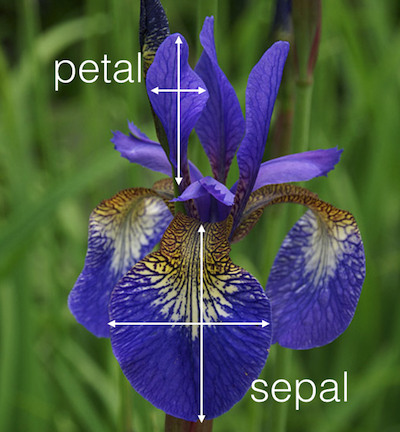
\includegraphics[width=0.3\linewidth]{iris} \caption{Iris plant with sepal and petal leaves}\label{fig:iris_pic}
\end{figure}

\scriptsize
<http://blog.kaggle.com/2015/04/22/scikit-learn-video-3-machine-learning-first-steps-with-the-iris-dataset/>

\end{block}

\end{frame}

\begin{frame}

\textbf{Set-up:} Training observations
\(\{(x_1, y_1), ..., (x_n, y_n)\}\) where the response variable \(Y\) is
categorical, e.g \(Y \in \mathcal{C} = \{0, 1, ..., 9\}\) or
\(Y \in \mathcal{C} = \{dog, cat,... ,horse\}\).

\textbf{Aim: } To \emph{build} a classifier \(f(x)\) that assigns a
class label from \(\mathcal{C}\) to a future unlabelled observation
\(x\) and to asses the \emph{uncertainty} in this classification.

\textbf{Performance measure:} Most popular is the misclassification
error rate (training and test version)..

\end{frame}

\begin{frame}

\begin{block}{Bayes classifier}

\begin{itemize}
\item
  The \emph{Bayes classifier assigns an observation to the most likely
  class}, given its predictor values.
\item
  Suppose we have a quantitative response value that can be a member in
  one of \(K\) classes
  \(\mathcal{C} = \{c_1, c_2, ..., c_k, ..., c_K\}\). Further, suppose
  these elements are numbered \(1, 2, ..., K\). The probability of that
  a new observation \(x_0\) belongs to class \(k\) is
  \[p_k(x_0) = \text{Pr}(Y=k | X=x_0), \quad k = 1, 2, ... K.\] This is
  the conditional class probability: the probability that \(Y=k\) given
  the observation \(x_0\).
\item
  Two-class example for two groups \(\{A, B\}\). A new observation
  \(x_0\) will be classified to \(A\) if
  \(\text{Pr}(Y=A | X=x_0) > 0.5\) and to class \(B\) otherwise.
\end{itemize}

\end{block}

\end{frame}

\begin{frame}

Given a continuous random vector \(X\) and categorical random variable
\(Y\), how do we get \(\text{Pr}(Y=k | X=x_0)\)?

\begin{center}
\colorbox{lightgray}{\begin{minipage}{10cm}
{\bf Bayes theorem}
\begin{align*}
P(Y=k \mid X= x) &= 
\frac{P({\bf X}={\bf x} \cap Y=k)}{f({\bf x})}\\
&= \frac{ f_k(x) \pi_k}{\sum_{l=1}^K  f_l(x) \pi_l}
\end{align*}
\end{minipage}}
\end{center}

Here \(f_k(x) = P(X=x \mid Y=k)\) is the pdf for \(X\) in class \(k\)
and \(\pi_k = P(Y=k)\) is the prior probability for class \(k\).

\end{frame}

\begin{frame}

\begin{block}{Properties of the Bayes classifier}

\begin{itemize}
\item
  It has the \emph{smallest test error rate}.
\item
  The class boundaries using the Bayes classifier is called the
  \emph{Bayes decision boundary}.
\item
  The overall Bayes error rate is given as
  \[1-\text{E}(\text{max} \text{Pr}(Y=j\mid X))\] where the expectation
  is over \(X\).
\item
  The Bayes error rate is comparable to the \emph{irreducible error} in
  the regression setting.
\item
  Caveat: we never (or very seldom) know the conditional distribution of
  \(Y\) given \(X\) for real data
\end{itemize}

\(\rightarrow\) The \(K\)-nearest neighbor classifier estimates this
conditional distribution and then classifies a new observation based on
this estimated probability.

\end{block}

\end{frame}

\begin{frame}

\begin{block}{K-nearest neighbour classifier}

\vspace{2mm} The \(K\)-nearest neighbour classifier (KNN) works in the
following way:

\begin{itemize}
\tightlist
\item
  Given a new observation \(x_0\) it searches for the \(K\) points in
  our training data that are closest to it (Euclidean distance).
\item
  These points make up the neighborhood of \(x_0\), \(\mathcal{N}_0\).
\item
  The point \(x_0\) is classified by taking a majority vote of the
  neighbors.
\item
  That means that \(x_0\) is classified to the most occurring class
  among its neighbors
  \[\text{Pr}(Y=j | X = x_0) = \frac{1}{K} \sum_{i \in \mathcal{N}_0} I(y_i = j).\]
\end{itemize}

\end{block}

\end{frame}

\begin{frame}

\begin{block}{A synthetic example}

\begin{itemize}
\item
  Simulate \(2\times 100\) observations from a bivariate normal
  distribution with mean vectors \(\mu_A = (1, 1)^T\),
  \(\mu_B = (3, 3)^T\), and covariance matrix
  \(\Sigma_A = \Sigma_B = \begin{pmatrix} 2\hspace{2mm} 0 \\ 0 \hspace{2mm} 2 \end{pmatrix}\).
\item
  Aim: Find a rule to classify a new observation to \(A\) or \(B\).
\end{itemize}

\begin{center}\includegraphics[width=0.55\linewidth]{4Classif_files/figure-beamer/knn-1} \end{center}

\end{block}

\end{frame}

\begin{frame}

\begin{itemize}
\tightlist
\item
  Assume we have a new observation \(X_0 = (x_{01}, x_{02})^T\) which we
  want to classify as belonging to the class \(A\) or \(B\).
\item
  To illustrate this problem we fit the \(K\)-nearest neighbor
  classifier to our simulated data set with \(K = 1, 3, 10\) and \(150\)
  (next slide).
\end{itemize}

\vspace{4mm}

Interpretation:

\begin{itemize}
\tightlist
\item
  The small colored dots show the predicted classes for an evenly-spaced
  grid.
\item
  The lines show the decision boundaries.
\item
  If our new observation falls into the region within the red decision
  boundary, it will be classified as \(A\). If it falls into the region
  within the green decision boundary, it will be classified as \(B\).
\end{itemize}

\end{frame}

\begin{frame}

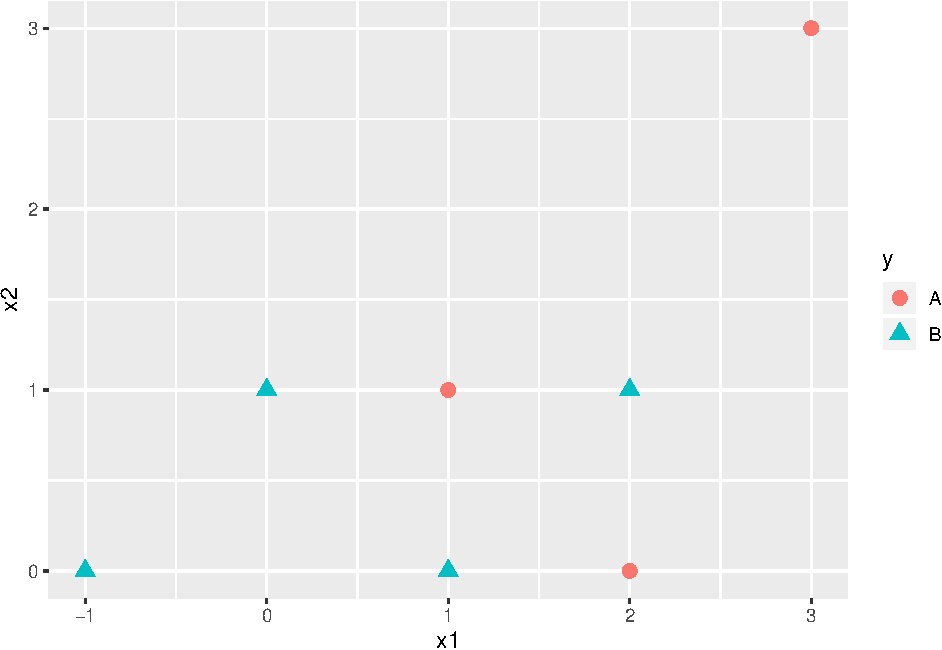
\includegraphics{4Classif_files/figure-beamer/unnamed-chunk-1-1.pdf}

\end{frame}

\begin{frame}

\begin{itemize}
\item
  The choice of \(K\) has a big influence on the result of our
  classification. For \(K=1\) the classification is made to the same
  class as the one nearest neighbor. As \(K\) gets very large, the
  decision boundary tends towards a straight line (which is the Bayes
  boundary in this set-up).
\item
  To find the optimal value of \(K\) the typical procedure is to try
  different values of \(K\) and then test the predictive power of the
  different classifiers, for example by cross-validation, which will be
  discussed in M5.
\item
  After trying all choices for \(K\) between 1 and 50, a few choices of
  \(K\) gave the smallest misclassification error rate, estimating by
  leave-one out cross-validation (see M5). The smallest error rate is
  equal to 0.165 (16.5\% misclassification).
\end{itemize}

\end{frame}

\begin{frame}

\begin{center}\includegraphics{4Classif_files/figure-beamer/knnerror1-1} \end{center}

\end{frame}

\begin{frame}

\begin{block}{Bias-variance trade-off in a classification setting}

\begin{itemize}
\item
  A too low value of \(K\) will give a very flexible classifier (with
  high variance and low bias) which will fit the training set too well
  (it will overfit) and make poor predictions for new observations.
\item
  Choosing a high value for \(K\) makes the classifier loose its
  flexibility and the classifier will have low variance but high bias.
\end{itemize}

\(\rightarrow\) Critical to the success of the classifier to choose the
correct level of flexibility (\(K\)).

\end{block}

\end{frame}

\begin{frame}

\begin{block}{The curse of dimensionality}

\begin{itemize}
\item
  The nearest neighbor classifier can be quite good if the number of
  predictor \(p\) is small and the number of observations \(n\) is
  large. We need enough close neighbors to make a good classification.
\item
  The effectiveness of the KNN classifier falls quickly when the
  dimension of the preditor space is high.
\item
  Why? Because the nearest neighbors tend to be far away in high
  dimensions and the method no longer is local. This is referred to as
  the \emph{curse of dimensionality}.
\end{itemize}

\end{block}

\end{frame}

\begin{frame}

\begin{block}{Synthetic example: what is the Bayes error?}

Suppose we have observations coming from two classes: \{{green},
{orange}\}, where
\[X_{\text{green}}\sim \mathcal{N}(-2, 1.5^2) \text{ and }
X_{\text{orange}}\sim \mathcal{N}(2, 1.5^2) \] and that the probability
of observing each class is equal.

\begin{itemize}
\tightlist
\item
  Where is the Bayes decision boundary here?
\item
  How can we calculate the Bayes error rate (intuitively- see the
  graph)?
\item
  What would you estimate the Bayes error rate to be?
\item
  What if someone constructs a classifier and it has a lower error rate
  than the Bayes error rate - is this possible?
\end{itemize}

\end{block}

\end{frame}

\begin{frame}

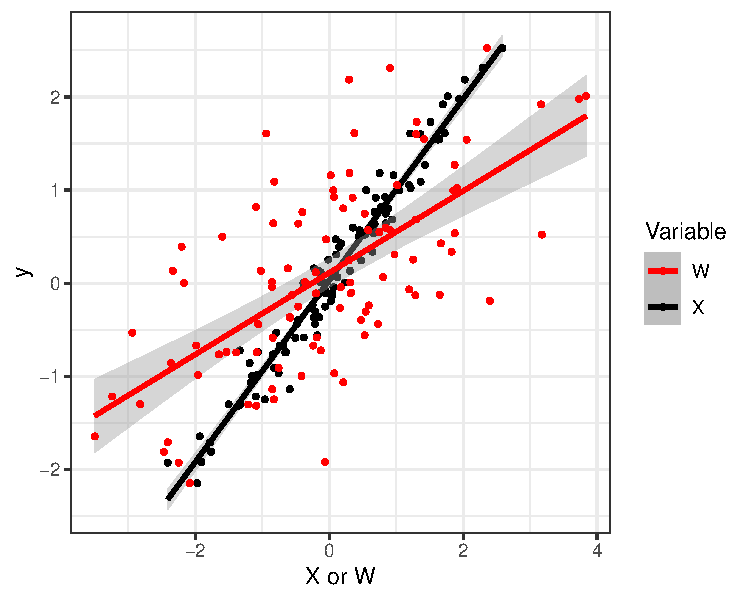
\includegraphics{4Classif_files/figure-beamer/unnamed-chunk-2-1.pdf}

\end{frame}

\begin{frame}[fragile]

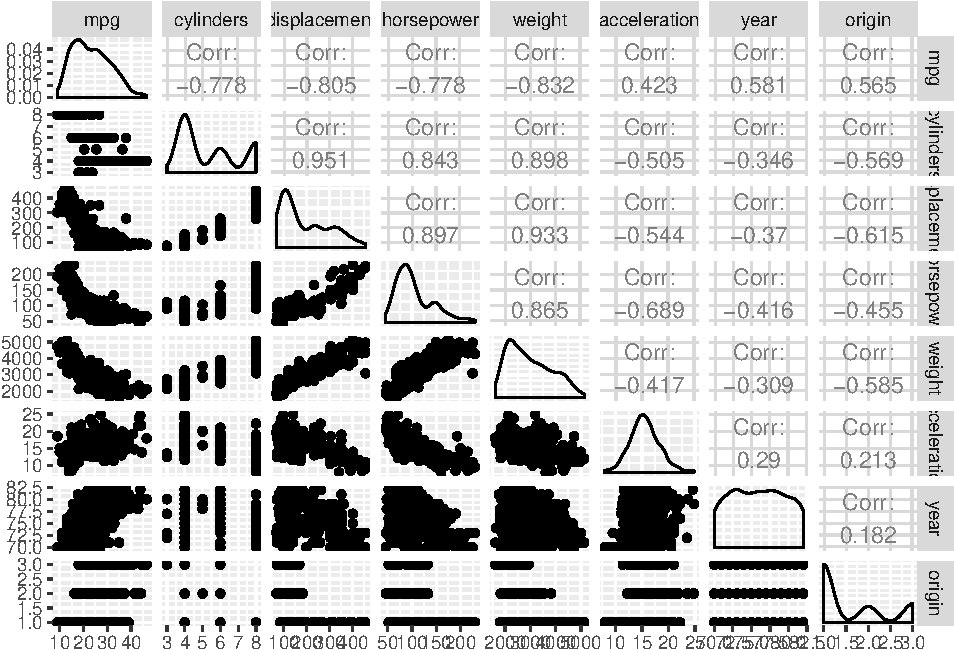
\includegraphics{4Classif_files/figure-beamer/unnamed-chunk-3-1.pdf}

Bayes error: \texttt{round(0.5*2*pnorm(0,mean=2,sd=1.5),2)}=0.09

\end{frame}

\begin{frame}

\begin{block}{Bayes decision rule - two paradigms}

The most popular approach to classication is to use the Bayes decision
rule with the 0/1 loss function= classify to the class with the largest
\(P(Y=k\mid X=x_0)\).

Two approaches:

\begin{itemize}
\item
  The \textbf{diagnostic paradigm}: We focus on \emph{directly}
  estimating the posterior distribution for the classes
  \(P(Y=k \mid X=x)\).
\item
  The \textbf{sampling paradigm}: There focus is on estimating the prior
  probabilities \(\pi_k\) for the classes and the class conditional
  distributions \(f_k(x)\). We classify to the class with the maximal
  product \(\pi_k f_k(x)\).
\end{itemize}

We \emph{first} look at the sampling paradigm - and then we need to
model the pdf for each class. Popular: the multivariate normal
distribution!

\end{block}

\end{frame}

\begin{frame}

\begin{block}{Univariate normal class distributions - the role of the
prior}

Suppose (again) we have observations coming from two classes: \{{green},
{orange}\}, where
\[X_{\text{green}}\sim \mathcal{N}(-2, 1.5^2) \text{ and }
X_{\text{orange}}\sim \mathcal{N}(2, 1.5^2) \]

In the figure below we have specified the prior probabilities to be
equal, \(\pi_1 = \pi_2 = 0.5\) and have plotted \(\pi_k f_k(x)\) for the
two classes.

The decision boundary is where the point of intersection of the two
lines is, because here \(\pi_1 f_1(x)=\pi_2 f_2(x)\). Thus all points to
left of the decision boundary will be classified as green and similarly,
all points to the right of the decision boundary will be classified as
orange.

\end{block}

\end{frame}

\begin{frame}

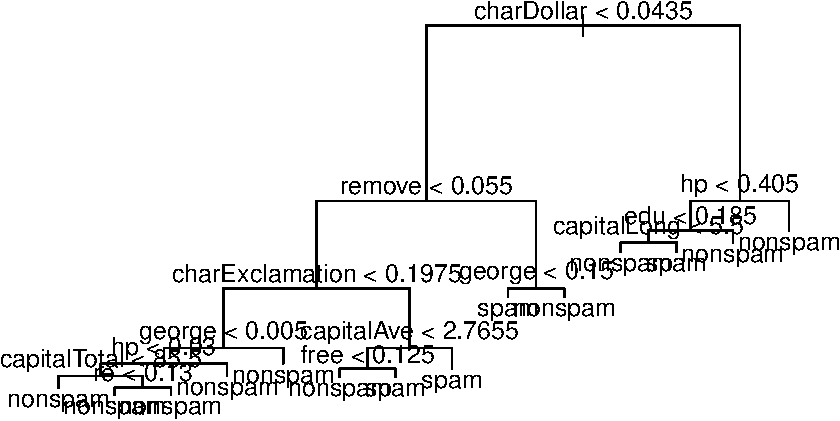
\includegraphics{4Classif_files/figure-beamer/unnamed-chunk-4-1.pdf}

\end{frame}

\begin{frame}

We now specify different priors, such that \(\pi_1 = 0.3\) and
\(\pi_2 = 0.7\). We see that this has affected the decision boundary,
which now has shifted to the left.

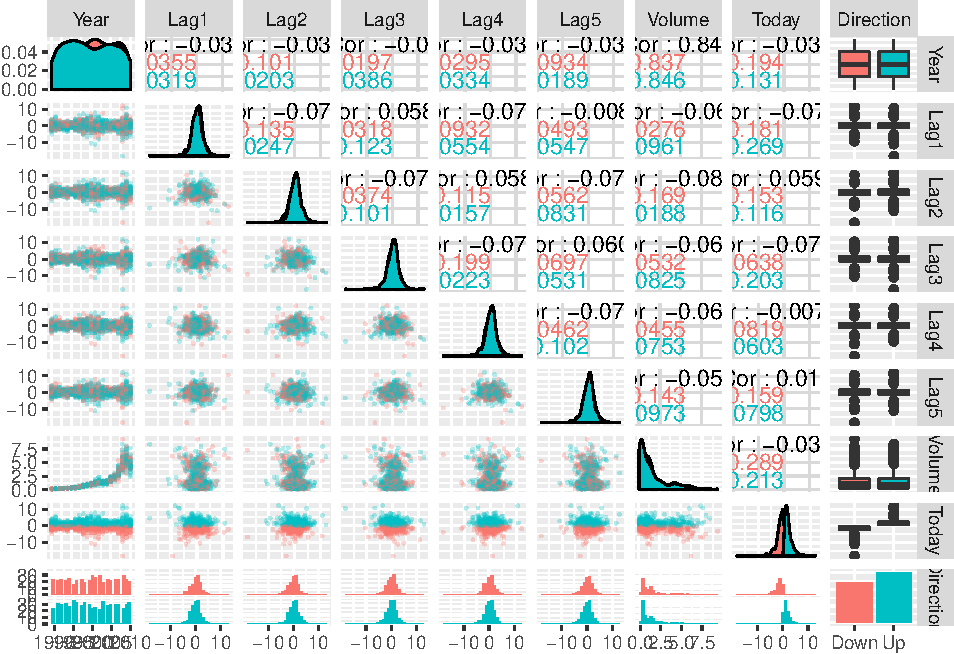
\includegraphics{4Classif_files/figure-beamer/unnamed-chunk-5-1.pdf}

\end{frame}

\begin{frame}{Linear and quadratic discriminant analysis}

\begin{block}{Linear discriminant analysis (LDA)}

Using Linear discriminant analysis we assume the class conditional
distributions are normal (Gaussian).

\begin{block}{Univariate (p=1)}

The univariate normal pdf
\[f(x) = \frac{1}{\sqrt{2\pi}\sigma} e^{-\frac{1}{2}\big(\frac{x-\mu}{\sigma}\big)^2},\]
has parameters \(\mu\) (mean) and \(\sigma\) (standard deviation).

Assume that we observe \(K\) classes, where each class conditional
distribution is normal, where the classes have mean \(\mu_k\) and
standard deviation \(\sigma_k\):
\[f_k(x) = \frac{1}{\sqrt{2\pi}\sigma_k} e^{-\frac{1}{2}\big(\frac{x-\mu_k}{\sigma_k}\big)^2}\]
With LDA we assume that all of the classes have the \emph{same standard
deviation} \(\sigma_k = \sigma\).

In addition we have prior class probabilites \(\pi_k=P(Y=k)\), so that
\(\sum_{k=1}^K \pi_k=1\).

\end{block}

\end{block}

\end{frame}

\begin{frame}

We can insert the expression for each class distribution into Bayes
formula to obtain the posterior probability
\(p_k(x) = P(Y = k | X = x)\):
\[p_k(x) = \frac{f_k({\bf x}) \pi_k}{f({\bf x})}=\frac{\pi_k \frac{1}{\sqrt{2\pi}\sigma} e^{-\frac{1}{2}\big(\frac{x-\mu_k}{\sigma}\big)^2}}{\sum_{l=1}^K \pi_l \frac{1}{\sqrt{2\pi}\sigma} e^{-\frac{1}{2}\big(\frac{x-\mu_l}{\sigma}\big)^2}} \]

Our rule is to classify to the class for which \(p_k(x)\) is largest.

It can be shown that this is equivalent to assigning \(x\) to the class
with the largest \emph{discriminant score} \(\delta_k(x)\):
\[\delta_k(x) = x\cdot \frac{\mu_k}{\sigma^2} - \frac{\mu_k^2}{2 \sigma^2}+\log(\pi_k).\]
This decision boundaries between the classes are \emph{linear} in \(x\).

\textbf{Q:} So, what do we need to use this result in practice?

\end{frame}

\begin{frame}

\begin{block}{Parameter estimators}

In real life situations we will not know the prior probabilities, the
class mean or standard deviation=need parameter estimators.

\begin{itemize}
\item
  Prior probability for class \(k\) is (often) estimated by taking the
  fraction of observations \(n_k\) (out of \(n\)) coming from class
  \(k\): \(\hat{\pi}_k = \frac{n_k}{n}.\)
\item
  The mean value for class \(k\) is simply the sample mean of all
  observations from class \(k\):
  \[\hat{\mu}_k = \frac{1}{n_k}\sum_{i:y_i=k} x_i.\]
\item
  The standard deviation: sample standard deviation across all classes:
  \[\hat{\sigma}^2=\frac{1}{n-K}\sum_{k=1}^K \sum_{i: y_i=k} (x_i-\hat{\mu}_k)^2 = \sum_{k=1}^K \frac{n_k - 1}{n - K} \cdot \hat{\sigma}_k^2.\]
  \(\hat{\sigma}_k\): estimated standard deviation of all observations
  from class \(k\).
\end{itemize}

\end{block}

\end{frame}

\begin{frame}[fragile]

\begin{block}{How would the estimation affect our misclassification
rate?}

If \(\mu_1=-2\), \(\mu_2=2\), \(\sigma=1.5\), \(\pi_1=\pi_2=0.5\) we
found that the class boundary is at 0 and the Bayes error is
\texttt{round(2*0.5*pnorm(0,2,1.5))}=0.09.

But, in a real life situation

\begin{itemize}
\tightlist
\item
  we estimate the class boundary
\item
  and we do not know the true distribution for the classes.
\end{itemize}

How can we then estimate the goodness of our estimator?

\end{block}

\end{frame}

\begin{frame}[fragile]

\begin{enumerate}
\def\labelenumi{\arabic{enumi}.}
\tightlist
\item
  Use the training set to estimate parameters and class boundary:
\item
  Use the test set to estimate misclassification rate.
\end{enumerate}

\footnotesize

\begin{Shaded}
\begin{Highlighting}[]
\NormalTok{n =}\StringTok{ }\DecValTok{1000}
\NormalTok{pi1 =}\StringTok{ }\NormalTok{pi2 =}\StringTok{ }\FloatTok{0.5}
\NormalTok{mu1 =}\StringTok{ }\DecValTok{-2}
\NormalTok{mu2 =}\StringTok{ }\DecValTok{2}
\NormalTok{sigma =}\StringTok{ }\FloatTok{1.5}
\KeywordTok{set.seed}\NormalTok{(}\DecValTok{1}\NormalTok{)}
\NormalTok{n1train =}\StringTok{ }\KeywordTok{rbinom}\NormalTok{(}\DecValTok{1}\NormalTok{, n, pi1)}
\NormalTok{n2train =}\StringTok{ }\NormalTok{n }\OperatorTok{-}\StringTok{ }\NormalTok{n1train}
\NormalTok{n1test =}\StringTok{ }\KeywordTok{rbinom}\NormalTok{(}\DecValTok{1}\NormalTok{, n, pi1)}
\NormalTok{n2test =}\StringTok{ }\NormalTok{n }\OperatorTok{-}\StringTok{ }\NormalTok{n1test}
\NormalTok{train1 =}\StringTok{ }\KeywordTok{rnorm}\NormalTok{(n1train, mu1, sigma)}
\NormalTok{train2 =}\StringTok{ }\KeywordTok{rnorm}\NormalTok{(n2train, mu2, sigma)}
\NormalTok{test1 =}\StringTok{ }\KeywordTok{rnorm}\NormalTok{(n1test, mu1, sigma)}
\NormalTok{test2 =}\StringTok{ }\KeywordTok{rnorm}\NormalTok{(n2test, mu2, sigma)}
\NormalTok{sigma2}\FloatTok{.1}\NormalTok{ =}\StringTok{ }\KeywordTok{var}\NormalTok{(train1)}
\NormalTok{sigma2}\FloatTok{.2}\NormalTok{ =}\StringTok{ }\KeywordTok{var}\NormalTok{(train2)}
\NormalTok{estsigma2 =}\StringTok{ }\NormalTok{((n1train }\OperatorTok{-}\StringTok{ }\DecValTok{1}\NormalTok{) }\OperatorTok{*}\StringTok{ }\NormalTok{sigma2}\FloatTok{.1} \OperatorTok{+}\StringTok{ }\NormalTok{(n2train }\OperatorTok{-}\StringTok{ }\DecValTok{1}\NormalTok{) }\OperatorTok{*}\StringTok{ }\NormalTok{sigma2}\FloatTok{.2}\NormalTok{)}\OperatorTok{/}\NormalTok{(n }\OperatorTok{-}\StringTok{ }
\StringTok{    }\DecValTok{2}\NormalTok{)}

\NormalTok{rule =}\StringTok{ }\FloatTok{0.5} \OperatorTok{*}\StringTok{ }\NormalTok{(}\KeywordTok{mean}\NormalTok{(train1) }\OperatorTok{+}\StringTok{ }\KeywordTok{mean}\NormalTok{(train2)) }\OperatorTok{+}\StringTok{ }\NormalTok{estsigma2 }\OperatorTok{*}\StringTok{ }\NormalTok{(}\KeywordTok{log}\NormalTok{(n2train}\OperatorTok{/}\NormalTok{n) }\OperatorTok{-}\StringTok{ }
\StringTok{    }\KeywordTok{log}\NormalTok{(n1train}\OperatorTok{/}\NormalTok{n))}\OperatorTok{/}\NormalTok{(}\KeywordTok{mean}\NormalTok{(train1) }\OperatorTok{-}\StringTok{ }\KeywordTok{mean}\NormalTok{(train2))}

\KeywordTok{c}\NormalTok{((}\KeywordTok{sum}\NormalTok{(train1 }\OperatorTok{>}\StringTok{ }\NormalTok{rule) }\OperatorTok{+}\StringTok{ }\KeywordTok{sum}\NormalTok{(train2 }\OperatorTok{<}\StringTok{ }\NormalTok{rule))}\OperatorTok{/}\NormalTok{n, (}\KeywordTok{sum}\NormalTok{(test1 }\OperatorTok{>}\StringTok{ }\NormalTok{rule) }\OperatorTok{+}\StringTok{ }\KeywordTok{sum}\NormalTok{(test2 }\OperatorTok{<}\StringTok{ }
\StringTok{    }\NormalTok{rule))}\OperatorTok{/}\NormalTok{n)}
\end{Highlighting}
\end{Shaded}

\begin{verbatim}
## [1] 0.105 0.115
\end{verbatim}

\normalsize

\end{frame}

\begin{frame}

\begin{block}{Training error rate}

the proportion of mistakes that are made if we apply classifier
\(\hat{f}\) to the training observations, i.e.
\(\hat{y}_i=\hat{f}(x_i)\).
\[\frac{1}{n}\sum_{i=1}^n \text{I}(y_i \neq \hat{y}_i).\] Here I is the
indicator function (to give our 0/1 loss) which is defined as:
\[\text{I}(a\neq\hat{a}) = \begin{cases} 1 \text{ if } a \neq \hat{a} \\ 0 \text{ else } \end{cases}\]
The indicator function counts the number of times our model has made a
wrong classification. The training error rate is the fraction of
misclassifications made on our training set.

A very low training error rate may imply overfitting.

\end{block}

\end{frame}

\begin{frame}

\begin{block}{Test error rate}

Here the fraction of misclassifications is calculated when our model is
applied on a test set. From what we have learned about regression we can
deduct that this gives a better indication of the true performance of
the classifier (than the training error).
\[\text{Ave}(I(y_0\neq \hat{y}_0))\] where the average is over all the
test observations \((x_0,y_0)\).

We assume that a \emph{good} classifier is a classifier that has a
\emph{low} test error.

\end{block}

\end{frame}

\begin{frame}

\begin{block}{The confusion matrix}

The confusion matrix is a table that can show the performance of
classifier, given that the true values are known.

We can make a confusion matrix from the training or test set, but will
in most cases do so for the test set only.

The rows represent the true classes, while the columns represent the
predicted classes. Inside the table we have counts (just labelled
``correct'' and ``wrong'' below - but should be numbers). The sum of the
diagonal is the total number of correct classifications. The sum of all
elements off the diagonal is the total number of misclassifications.

Predicted 1

Predicted 2

\ldots{}

Predicted K

True 1

correct

wrong

\ldots{}

wrong

True 2

wrong

correct

\ldots{}

wrong

\ldots{}

\ldots{}

\ldots{}

\ldots{}

\ldots{}

True K

wrong

wrong

\ldots{}

correct

\end{block}

\end{frame}

\begin{frame}[fragile]

The confusion matrix can be obtained in \texttt{R} by using the
\texttt{table} function with the predicted classes and the true classes
need to be given as function arguments, or directly using the
\texttt{caret} package.

We will soon come back to the special case of two classes - where we may
think of this as ``-'' (non disease) and ``+'' (disease).

\end{frame}

\begin{frame}

\begin{block}{Multivariate LDA (p\textgreater{}1)}

Linear discriminant analysis can be generalized to situations when
\(p>1\) covariates are used. The decision boundaries are still linear.

The multivariate normal distribution function:
\[f(x) = \frac{1}{(2 \pi)^{p/2}|\boldsymbol{\Sigma}|^{1/2}}\exp({-\frac{1}{2}({\bf x}-\boldsymbol\mu)^T \boldsymbol{\Sigma}^{-1}({\bf x}-\boldsymbol\mu)})\]

This gives the following expression for the discriminant function:
\[\delta_k(x) = {\bf x}^T \boldsymbol{\Sigma}^{-1}\boldsymbol\mu_k - \frac{1}{2}\boldsymbol\mu_k^T \boldsymbol{\Sigma}^{-1}\boldsymbol\mu_k + \log \pi_k.\]

\end{block}

\end{frame}

\begin{frame}

Some details on the derivation of the discriminant function - when
\(K=2\) classes, and the classes are denoted \(0\) and \(1\)

\[P(Y=0 | X={\bf x}) = P(Y=1 | X={\bf x})\]
\[\frac{\pi_0f_0(x)}{\pi_0f_0(x)+\pi_1f_1(x)} = \frac{\pi_1f_0(1)}{\pi_0f_0(x)+\pi_1f_1(x)} \]
\[\pi_0 f_0({\bf x}) = \pi_1 f_1({\bf x})\]
\[\pi_0\frac{1}{(2 \pi)^{p/2}|\boldsymbol{\Sigma}|^{1/2}}
e^{\frac{1}{2}({\bf x}-\boldsymbol{\mu}_0)^T \boldsymbol{\Sigma}^{-1}({\bf x}-\boldsymbol{\mu}_0)} =  \pi_1\frac{1}{(2 \pi)^{p/2}|\boldsymbol{\Sigma}|^{1/2}}e^{\frac{1}{2}({\bf x}-\boldsymbol{\mu}_1)^T \boldsymbol{\Sigma}^{-1}({\bf x}-\boldsymbol{\mu}_1)} \]
\[log(\pi_0) -\frac{1}{2}({\bf x}-\boldsymbol{\mu}_0)^T \boldsymbol{\Sigma}^{-1}({\bf x}-\boldsymbol{\mu}_0) = log(\pi_1) -\frac{1}{2}({\bf x}-\boldsymbol{\mu}_1)^T \boldsymbol{\Sigma}^{-1}({\bf x}-\boldsymbol{\mu}_1) \]
\[log(\pi_0)  -\frac{1}{2}x^T\boldsymbol{\Sigma}^{-1}{\bf x} + {\bf x}^T\boldsymbol{\Sigma}^{-1}\boldsymbol{\mu}_0 - \frac{1}{2}\boldsymbol{\mu}_0^T\boldsymbol{\Sigma}^{-1}\boldsymbol{\mu}_0 = log(\pi_1)  -\frac{1}{2}{\bf x}^T\boldsymbol{\Sigma}^{-1}{\bf x} + {\bf x}^T\boldsymbol{\Sigma}^{-1}\boldsymbol{\mu}_1 - \frac{1}{2}\boldsymbol{\mu}_1^T\boldsymbol{\Sigma}^{-1}\boldsymbol{\mu}_1 \]
\[log(\pi_0) + {\bf x}^T\boldsymbol{\Sigma}^{-1}\boldsymbol{\mu}_0 - \frac{1}{2}\boldsymbol{\mu}_0^T\boldsymbol{\Sigma}^{-1}\boldsymbol{\mu}_0 = log(\pi_1) + {\bf x}^T\boldsymbol{\Sigma}^{-1}\boldsymbol{\mu}_1 - \frac{1}{2}\mu_1^T\boldsymbol{\Sigma}^{-1}\boldsymbol{\mu}_1\]
\[\delta_0({\bf x}) = \delta_1({\bf x}) \]

\end{frame}

\begin{frame}

\textbf{Estimators for p\textgreater{}1:}

\begin{itemize}
\item
  Prior probability for class \(k\) (unchanged from p=1):
  \(\hat{\pi}_k = \frac{n_k}{n}.\)
\item
  The mean value for class \(k\) is simply the sample mean of all
  observations from class \(k\) (but now these are vectors):
  \[\hat{\boldsymbol{\mu}}_k = \frac{1}{n_k}\sum_{i:y_i=k} {\bf X}_i.\]
\item
  The covariance matrices for each class:
  \[\hat{\boldsymbol{\Sigma}}_k=\frac{1}{n_k-1}\sum_{i:y_i=k} ({\bf X}_i-\hat{\boldsymbol{\mu}}_k ) ({\bf X}_i-\hat{\boldsymbol{\mu}}_k)^T\]
\item
  Pooled version:
  \[\hat{\boldsymbol{\Sigma}}= \sum_{k=1}^K \frac{n_k - 1}{n - K} \cdot \hat{\boldsymbol{\Sigma}}_k.\]
\end{itemize}

Optional:
\href{https://www.math.ntnu.no/emner/TMA4268/2018v/notes/ProofMeanS.pdf}{Proof
that the estimator \(\hat{\boldsymbol{\Sigma}}_k\) is unbiased for each
class (from TMA4267)}. Proof for pooled version not provided.

\end{frame}

\begin{frame}

\begin{block}{Posterior probabilites}

Sometimes the probability that an observation comes from a class \(k\)
is more interesting than the actual classification itself. These class
probabilities can be estimated from the priors and class conditional
distributions, or from the discriminant functions:

\begin{align*}\hat{P}(Y=k | X=x)&=
\frac{\hat{\pi}_k \cdot \frac{1}{(2 \pi)^{p/2}|\hat{\boldsymbol{\Sigma}}|^{1/2}} \exp(-\frac{1}{2}
({\bf x}-\hat{\boldsymbol\mu}_k)^T \hat{\boldsymbol{\Sigma}}^{-1}
({\bf x}-\hat{\boldsymbol\mu}_k))}
{\sum_{l=1}^K \hat{\pi}_l 
\frac{1}{(2 \pi)^{p/2}|\hat{\boldsymbol{\Sigma}}|^{1/2}}
\exp(-\frac{1}{2}
({\bf x}-\hat{\boldsymbol\mu}_l)^T 
\hat{\boldsymbol{\Sigma}}^{-1}
({\bf x}-\hat{\boldsymbol\mu}_l))}\\
&=
\frac{e^{\hat{\delta}_k(x)}}{\sum_{l=1}^K e^{\hat{\delta}_l(x)}}.\end{align*}

\end{block}

\end{frame}

\begin{frame}

\begin{block}{Quadratic Discriminant Analysis (QDA)}

In quadratic discriminant analysis we assume that the distributions of
the classes is multivariate normal (Gaussian), but with covariance
matrix \(\boldsymbol{\Sigma}_k\) for each class.

The discriminant functions are now given by:

\begin{align*} \delta_k(x) &= -\frac{1}{2}(x-\mu_k)^T \boldsymbol{\Sigma}_k^{-1}(x-\mu_k)-\frac{1}{2}\log |\boldsymbol{\Sigma}_k| + \log \pi_k \\ &= -\frac{1}{2} x^T \boldsymbol{\Sigma}_k^{-1}x + x^T \boldsymbol{\Sigma}_k^{-1}\mu_k - \frac{1}{2} \mu_k^T \boldsymbol{\Sigma}_k^{-1}\mu_k - \frac{1}{2}\log |\boldsymbol{\Sigma}_k | + \log \pi_k.\end{align*}

These decision boundaries are \emph{quadratic} functions of \(x\).

\end{block}

\end{frame}

\begin{frame}

\begin{block}{LDA vs QDA}

In QDA we are allowed for the covariance matrices to be different for
the classes, but for LDA they are assumed to be the same, so QDA is more
flexible than LDA.

\textbf{Q:}

\begin{itemize}
\tightlist
\item
  But, if the covariance matrices in theory are equal - will they not be
  estimated equal?
\item
  Should we not always prefer QDA to LDA?
\end{itemize}

\end{block}

\end{frame}

\begin{frame}

\textbf{A:}

Explanation similar to a ``Bias-variance trade-off'':

If the assumption of equal covariance matrices is wrong

\begin{itemize}
\tightlist
\item
  then LDA may suffer from high bias for the parameter estimators.
\item
  and QDA is better off. But, for small sample sizes the covariance
  matrices might be poorly estimated (high variance of estimators).
\end{itemize}

If the number of covariates is high:

\begin{itemize}
\tightlist
\item
  then QDA requires estimating \(K\cdot p \cdot (p+1)/2\) parameters,
\item
  while LDA only requires \(p\cdot(p+1)/2\).
\end{itemize}

Therefore, LDA is less flexible than QDA and might therefore have much
less variance.

\end{frame}

\begin{frame}

\begin{block}{Naive Bayes (optional)}

This is method that is popular when \(p\) is large.

In Naive Bayes (Idiot's Bayes) we assume that each class density is the
product of marginal densities - i.e.~inputs are conditionally
independent in each class. \[f_k(x)=\prod_{j=1}^p f_{kj}(x_j)\] This is
generally not true, but it simplifies the estimation dramatically.

The original naive Bayes used univariate normal marginal distributions,
but generalizations can be made.

Instead of estimating a full covariance matrix, only the diagonal
elements are estimated.

This method often produces good results, even though the joint pdf is
not the product of the marginal pdf. This might be because we are not
focussing on estimation of class pdfs, but class boundaries.

\end{block}

\end{frame}

\begin{frame}[fragile]

\begin{block}{Example: Classification of iris plants}

We will use \texttt{sepal\ width} and \texttt{sepal\ length} to build a
classificator, here 50 observations from each class available.

\begin{Shaded}
\begin{Highlighting}[]
\KeywordTok{attach}\NormalTok{(iris)}
\KeywordTok{library}\NormalTok{(class)}
\KeywordTok{library}\NormalTok{(MASS)}
\KeywordTok{library}\NormalTok{(ggplot2)}
\KeywordTok{library}\NormalTok{(dplyr)}
\KeywordTok{kable}\NormalTok{(}\KeywordTok{head}\NormalTok{(iris), }\DataTypeTok{format =}\NormalTok{ whichformat)}
\end{Highlighting}
\end{Shaded}

Sepal.Length

Sepal.Width

Petal.Length

Petal.Width

Species

5.1

3.5

1.4

0.2

setosa

4.9

3.0

1.4

0.2

setosa

4.7

3.2

1.3

0.2

setosa

4.6

3.1

1.5

0.2

setosa

5.0

3.6

1.4

0.2

setosa

5.4

3.9

1.7

0.4

setosa

\end{block}

\end{frame}

\begin{frame}[fragile]

\begin{Shaded}
\begin{Highlighting}[]
\NormalTok{iris0_plot =}\StringTok{ }\KeywordTok{ggplot}\NormalTok{(iris, }\KeywordTok{aes}\NormalTok{(}\DataTypeTok{x =}\NormalTok{ Sepal.Width, }\DataTypeTok{y =}\NormalTok{ Sepal.Length, }\DataTypeTok{color =}\NormalTok{ Species)) }\OperatorTok{+}\StringTok{ }
\StringTok{    }\KeywordTok{geom_point}\NormalTok{(}\DataTypeTok{size =} \FloatTok{2.5}\NormalTok{)}
\NormalTok{iris0_plot}
\end{Highlighting}
\end{Shaded}

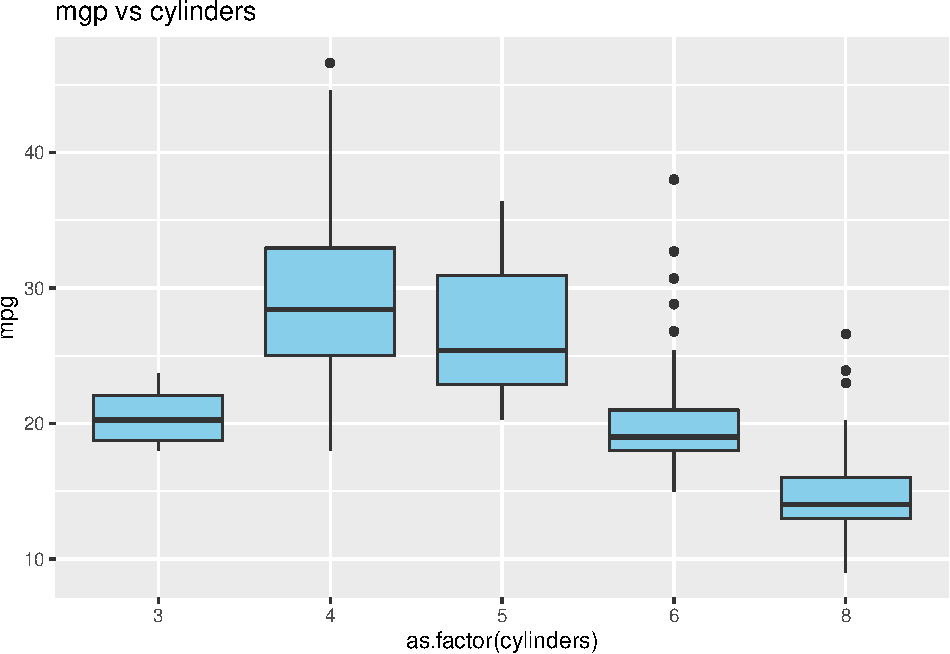
\includegraphics{4Classif_files/figure-beamer/unnamed-chunk-8-1.pdf}

\end{frame}

\begin{frame}[fragile]

\begin{block}{Iris: LDA}

\begin{Shaded}
\begin{Highlighting}[]
\CommentTok{# reporting on parameter estimates}

\NormalTok{grS =}\StringTok{ }\KeywordTok{cbind}\NormalTok{(iris[iris}\OperatorTok{$}\NormalTok{Species }\OperatorTok{==}\StringTok{ "setosa"}\NormalTok{, }\DecValTok{1}\OperatorTok{:}\DecValTok{2}\NormalTok{])}
\NormalTok{grVe =}\StringTok{ }\KeywordTok{cbind}\NormalTok{(iris[iris}\OperatorTok{$}\NormalTok{Species }\OperatorTok{==}\StringTok{ "versicolor"}\NormalTok{, }\DecValTok{1}\OperatorTok{:}\DecValTok{2}\NormalTok{])}
\NormalTok{grVi =}\StringTok{ }\KeywordTok{cbind}\NormalTok{(iris[iris}\OperatorTok{$}\NormalTok{Species }\OperatorTok{==}\StringTok{ "virginica"}\NormalTok{, }\DecValTok{1}\OperatorTok{:}\DecValTok{2}\NormalTok{])}
\NormalTok{nk =}\StringTok{ }\KeywordTok{dim}\NormalTok{(grS)[}\DecValTok{1}\NormalTok{]}
\KeywordTok{apply}\NormalTok{(grS, }\DecValTok{2}\NormalTok{, mean)}
\end{Highlighting}
\end{Shaded}

\begin{verbatim}
## Sepal.Length  Sepal.Width 
##        5.006        3.428
\end{verbatim}

\begin{Shaded}
\begin{Highlighting}[]
\NormalTok{cS =}\StringTok{ }\KeywordTok{cov}\NormalTok{(grS)}
\KeywordTok{apply}\NormalTok{(grVe, }\DecValTok{2}\NormalTok{, mean)}
\end{Highlighting}
\end{Shaded}

\begin{verbatim}
## Sepal.Length  Sepal.Width 
##        5.936        2.770
\end{verbatim}

\begin{Shaded}
\begin{Highlighting}[]
\NormalTok{cVe =}\StringTok{ }\KeywordTok{cov}\NormalTok{(grVe)}
\KeywordTok{apply}\NormalTok{(grVi, }\DecValTok{2}\NormalTok{, mean)}
\end{Highlighting}
\end{Shaded}

\begin{verbatim}
## Sepal.Length  Sepal.Width 
##        6.588        2.974
\end{verbatim}

\begin{Shaded}
\begin{Highlighting}[]
\NormalTok{cVi =}\StringTok{ }\KeywordTok{cov}\NormalTok{(grVi)}
\NormalTok{C =}\StringTok{ }\NormalTok{(nk }\OperatorTok{-}\StringTok{ }\DecValTok{1}\NormalTok{) }\OperatorTok{*}\StringTok{ }\NormalTok{(cS }\OperatorTok{+}\StringTok{ }\NormalTok{cVe }\OperatorTok{+}\StringTok{ }\NormalTok{cVi)}\OperatorTok{/}\NormalTok{(}\KeywordTok{dim}\NormalTok{(iris)[}\DecValTok{1}\NormalTok{] }\OperatorTok{-}\StringTok{ }\DecValTok{3}\NormalTok{)}
\NormalTok{C}
\end{Highlighting}
\end{Shaded}

\begin{verbatim}
##              Sepal.Length Sepal.Width
## Sepal.Length   0.26500816  0.09272109
## Sepal.Width    0.09272109  0.11538776
\end{verbatim}

\begin{Shaded}
\begin{Highlighting}[]
\KeywordTok{eigen}\NormalTok{(C)}
\end{Highlighting}
\end{Shaded}

\begin{verbatim}
## eigen() decomposition
## $values
## [1] 0.30933556 0.07106036
## 
## $vectors
##            [,1]       [,2]
## [1,] -0.9022004  0.4313171
## [2,] -0.4313171 -0.9022004
\end{verbatim}

\end{block}

\end{frame}

\begin{frame}

\includegraphics{4Classif_files/figure-beamer/irislda-1.pdf}

\end{frame}

\begin{frame}

\begin{block}{Iris: QDA}

\includegraphics{4Classif_files/figure-beamer/irisqda-1.pdf}

\end{block}

\end{frame}

\begin{frame}[fragile]

\begin{block}{Iris: compare LDA and QDA}

We now want to compare the predictive performance of our two
classifiers. We do this by dividing the original \texttt{iris} data set,
randomly, into train and test samples of equal size:

\begin{Shaded}
\begin{Highlighting}[]
\KeywordTok{set.seed}\NormalTok{(}\DecValTok{1}\NormalTok{)}
\NormalTok{train =}\StringTok{ }\KeywordTok{sample}\NormalTok{(}\DecValTok{1}\OperatorTok{:}\DecValTok{150}\NormalTok{, }\DecValTok{75}\NormalTok{)}

\NormalTok{iris_train =}\StringTok{ }\NormalTok{iris[train, ]}
\NormalTok{iris_test =}\StringTok{ }\NormalTok{iris[}\OperatorTok{-}\NormalTok{train, ]}

\NormalTok{iris_lda2 =}\StringTok{ }\KeywordTok{lda}\NormalTok{(Species }\OperatorTok{~}\StringTok{ }\NormalTok{Sepal.Length }\OperatorTok{+}\StringTok{ }\NormalTok{Sepal.Width, }\DataTypeTok{data =}\NormalTok{ iris_train, }
    \DataTypeTok{prior =} \KeywordTok{c}\NormalTok{(}\DecValTok{1}\NormalTok{, }\DecValTok{1}\NormalTok{, }\DecValTok{1}\NormalTok{)}\OperatorTok{/}\DecValTok{3}\NormalTok{)}
\end{Highlighting}
\end{Shaded}

\end{block}

\end{frame}

\begin{frame}[fragile]

\begin{Shaded}
\begin{Highlighting}[]
\CommentTok{# Training error}
\KeywordTok{table}\NormalTok{(}\KeywordTok{predict}\NormalTok{(iris_lda2, }\DataTypeTok{newdata =}\NormalTok{ iris_train)}\OperatorTok{$}\NormalTok{class, iris_train}\OperatorTok{$}\NormalTok{Species)}
\end{Highlighting}
\end{Shaded}

\begin{verbatim}
##             
##              setosa versicolor virginica
##   setosa         27          0         0
##   versicolor      1         15         8
##   virginica       0          5        19
\end{verbatim}

\begin{Shaded}
\begin{Highlighting}[]
\CommentTok{# Test error}
\NormalTok{iris_lda2_predict =}\StringTok{ }\KeywordTok{predict}\NormalTok{(iris_lda2, }\DataTypeTok{newdata =}\NormalTok{ iris_test)}
\KeywordTok{table}\NormalTok{(iris_lda2_predict}\OperatorTok{$}\NormalTok{class, iris}\OperatorTok{$}\NormalTok{Species[}\OperatorTok{-}\NormalTok{train])}
\end{Highlighting}
\end{Shaded}

\begin{verbatim}
##             
##              setosa versicolor virginica
##   setosa         22          0         0
##   versicolor      0         22        11
##   virginica       0          8        12
\end{verbatim}

\end{frame}

\begin{frame}

The LDA classifier has a training error rate of 15/75, that is 20 \%.
When tested on a new set it correctly classified 24+13+23 times and
misclassified 15 times. This gives a misclassification rate of
\[\text{Test error}_\text{LDA}  = \frac{15}{75} =0.2.\]

Using a different division into training and test set will give (small)
changes to these numbers.

\end{frame}

\begin{frame}[fragile]

\begin{block}{Iris: training and test error for QDA}

\begin{Shaded}
\begin{Highlighting}[]
\NormalTok{iris_qda2 =}\StringTok{ }\KeywordTok{qda}\NormalTok{(Species }\OperatorTok{~}\StringTok{ }\NormalTok{Sepal.Length }\OperatorTok{+}\StringTok{ }\NormalTok{Sepal.Width, }\DataTypeTok{data =}\NormalTok{ iris_train, }
    \DataTypeTok{prior =} \KeywordTok{c}\NormalTok{(}\DecValTok{1}\NormalTok{, }\DecValTok{1}\NormalTok{, }\DecValTok{1}\NormalTok{)}\OperatorTok{/}\DecValTok{3}\NormalTok{)}
\end{Highlighting}
\end{Shaded}

Important: use the same division into training and test set for methods
we want to compare.

\end{block}

\end{frame}

\begin{frame}[fragile]

\begin{Shaded}
\begin{Highlighting}[]
\CommentTok{# Training error}
\KeywordTok{table}\NormalTok{(}\KeywordTok{predict}\NormalTok{(iris_qda2, }\DataTypeTok{newdata =}\NormalTok{ iris_train)}\OperatorTok{$}\NormalTok{class, iris_train}\OperatorTok{$}\NormalTok{Species)}
\end{Highlighting}
\end{Shaded}

\begin{verbatim}
##             
##              setosa versicolor virginica
##   setosa         28          0         0
##   versicolor      0         16         9
##   virginica       0          4        18
\end{verbatim}

\begin{Shaded}
\begin{Highlighting}[]
\CommentTok{# Test error}
\NormalTok{iris_qda2_predict =}\StringTok{ }\KeywordTok{predict}\NormalTok{(iris_qda2, }\DataTypeTok{newdata =}\NormalTok{ iris_test)}
\KeywordTok{table}\NormalTok{(iris_qda2_predict}\OperatorTok{$}\NormalTok{class, iris}\OperatorTok{$}\NormalTok{Species[}\OperatorTok{-}\NormalTok{train])}
\end{Highlighting}
\end{Shaded}

\begin{verbatim}
##             
##              setosa versicolor virginica
##   setosa         22          0         0
##   versicolor      0         18        12
##   virginica       0         12        11
\end{verbatim}

\end{frame}

\begin{frame}

The QDA classifier has a training error rate of \(16\%\). When tested on
a new set, the misclassification error rate was
\[\text{Test error}_\text{QDA}  = \frac{18}{75}=.24\]

The LDA classifier has given the smallest test error for classifying
iris plants based on sepal width and sepal length for our test set and
should be preferred in this case.

\begin{enumerate}
\def\labelenumi{\arabic{enumi}.}
\tightlist
\item
  Would another division of the data into training and test set give the
  same conclusion (that LDA is better than QDA for this data set)? (A:
  Not necessarily, but probably.)
\end{enumerate}

We will look into other choice than dividing into one training and one
test set in Module 5 (crossvalidation).

\begin{enumerate}
\def\labelenumi{\arabic{enumi}.}
\setcounter{enumi}{1}
\tightlist
\item
  What about the other two covariates? Would adding them to the model (4
  covariates) give a better classification rule? (A: Probably. Try if
  you want.)
\end{enumerate}

\end{frame}

\begin{frame}

\begin{block}{Fishers idea (Optional)}

In 1936 R. A. Fisher developed LDA.

\begin{itemize}
\tightlist
\item
  His aim was to find a linear combination of the explanatory variables
  which \emph{maximized the ratio of its between class to within class
  variance}.
\item
  In this way the observations are transformed so that they are
  separated as much as possible.
\item
  His approach has the advantage that it is suited for visual inspection
  and graphical description , it ``separates'' the populations.
\end{itemize}

Let the between-class variance be denoted
\(\boldsymbol{B}=\sum_{m=1}^{M}(\boldsymbol{\mu}_{m}- \bar{\boldsymbol{\mu}})(\boldsymbol{\mu}_{m}-\bar{\boldsymbol{\mu}})^{T}\),
where \(\boldsymbol{\mu}_{m}\) denotes the mean of class \(\omega_{m}\)
and \(\bar{\boldsymbol{\mu}}\) the overall mean.

The within-class variance is assumed equal for all classes and is
denoted \(\boldsymbol{\Sigma}\) (\(\boldsymbol{\Sigma}\) is assumed to
have full rank).

\end{block}

\end{frame}

\begin{frame}

The linear combination \(\boldsymbol{l}^{T}\boldsymbol{X}\) that
maximize
\({\boldsymbol{l}^{T}\boldsymbol{B}\boldsymbol{l}}/{\boldsymbol{l}^{T}\boldsymbol{\Sigma}\boldsymbol{l}}\)
under the constraint that
\(\boldsymbol{l}^{T}\boldsymbol{\Sigma}\boldsymbol{l}=1\) is found to be
the scaled eigenvectors of \(\boldsymbol{\Sigma}^{-1}\boldsymbol{B}\)
corresponding to the nonzero eigenvalues of
\(\boldsymbol{\Sigma}^{-1}\boldsymbol{B}\). The eigenvector
corresponding to the largest eigenvalue defines the first discriminant
\(\boldsymbol{l}_{1}^{T}\boldsymbol{X}\). The second linear discriminant
\(\boldsymbol{l}_{2}^{T}\boldsymbol{X}\) is constructed from the
eigenvector corresponding to the second largest eigenvalue and so on.
(We also have
\(Cov(\boldsymbol{l}_{j}^{T}\boldsymbol{X},\boldsymbol{l}_{i}^{T}\boldsymbol{X})=0\)
for \(i \ne j\) and \(Var(\boldsymbol{l}_{j}^{T}\boldsymbol{X})=1\).)

\end{frame}

\begin{frame}

The number of linear discriminants equals the number of nonzero
eigenvalues. Observations are assigned to the class of the nearest
(Euclidean distance) class mean in the discriminant space.

This equals classification to the nearest Mahalanobis distance
population mean in the input space. Again, the parameters
\(\boldsymbol{\mu}_{i}\) and \(\boldsymbol{\Sigma}\) and the
between-class variance \(\boldsymbol{B}\) are usually unavailable.
Replacing the parameters by estimates from the training set leads to
Fisher's sample linear discriminants.

\end{frame}

\begin{frame}{Diagnostic paradigm}

Remember:

\begin{itemize}
\item
  The \textbf{diagnostic paradigm}: We focus on \emph{directly}
  estimating the posterior distribution for the classes
  \(P(Y=k \mid X=x)\).
\item
  The \textbf{sampling paradigm}: There focus is on estimating the prior
  probabilities for the classes and the class conditional distributions.
  We classify to the class with the maximal product \(\pi_k f_k(x)\).
\end{itemize}

Now we move to the \emph{diagnostic paradigm} and the \(K\)-nearest
neighbor classifier.

The \(K\)-nearest neighbour classifier estimates \(P(Y=k \mid X=x)\) and
classifies a new observation based on this estimated probability

\end{frame}

\begin{frame}

\begin{block}{Synthetic example for KNN classification}

Consider a two-class example, and equal class prior probabilites.

A new observation \(x_0\) will be classified to \(A\) if
\(P(Y=A | X=x_0) > 0.5\) and to class \(B\) otherwise.

\begin{itemize}
\tightlist
\item
  The figure below shows a plot of 100 observations from two classes
  \(A\) (red dots) and \(B\) (turquoise dots),
\item
  simulated from a bivariate normal distribution with mean vectors
  \(\mu_A = (1, 1)^T\) and \(\mu_B = (3, 3)^T\) and a covariance matrix
  \(\Sigma_A = \Sigma_B = \begin{pmatrix} 2\hspace{2mm} 0 \\ 0 \hspace{2mm} 2 \end{pmatrix}\).
\item
  We want to find a rule to classify a new observation to class \(A\) or
  \(B\).
\end{itemize}

\end{block}

\end{frame}

\begin{frame}

\includegraphics{4Classif_files/figure-beamer/synthAB-1.pdf}

\end{frame}

\begin{frame}[fragile]

\textbf{Remark:} since the truth is known here we can calculate the
Bayes boundary and the Bayes error.

Since we have bivariate normal class distributions with common
covariance matrix, the optimal boundary is given by LDA. The boundary
will be at \(\delta_A({\bf x})=\delta_B({\bf x})\), where
\(\delta_A({\bf x})= {\bf x}^T \boldsymbol{\Sigma}^{-1}\boldsymbol\mu_A - \frac{1}{2}\boldsymbol\mu_A^T \boldsymbol{\Sigma}^{-1}\boldsymbol\mu_A + \log \pi_A\),
and for \(\delta_B({\bf x})\) with \(\boldsymbol\mu_B\).

\[{\bf x}^T \boldsymbol{\Sigma}^{-1}\boldsymbol\mu_A - \frac{1}{2}\boldsymbol\mu_A^T \boldsymbol{\Sigma}^{-1}\boldsymbol\mu_A + \log \pi_A={\bf x}^T \boldsymbol{\Sigma}^{-1}\boldsymbol\mu_B - \frac{1}{2}\boldsymbol\mu_B^T \boldsymbol{\Sigma}^{-1}\boldsymbol\mu_B + \log \pi_B\]

\[{\bf x}^T\boldsymbol{\Sigma}^{-1}(\boldsymbol\mu_A -\boldsymbol\mu_B)-\frac{1}{2}\boldsymbol\mu_A^T \boldsymbol{\Sigma}^{-1}\boldsymbol\mu_A +\frac{1}{2}\boldsymbol\mu_B^T \boldsymbol{\Sigma}^{-1}\boldsymbol\mu_B +\log \pi_A-\log \pi_B=0\]

Inserting numerical values gives: \(-x_1-x_2+4=0\), and boundary
\(x_2=4-x_1\).

\begin{Shaded}
\begin{Highlighting}[]
\NormalTok{muA =}\StringTok{ }\KeywordTok{matrix}\NormalTok{(}\KeywordTok{c}\NormalTok{(}\DecValTok{1}\NormalTok{, }\DecValTok{1}\NormalTok{), }\DataTypeTok{ncol =} \DecValTok{1}\NormalTok{)}
\NormalTok{muB =}\StringTok{ }\KeywordTok{matrix}\NormalTok{(}\KeywordTok{c}\NormalTok{(}\DecValTok{3}\NormalTok{, }\DecValTok{3}\NormalTok{), }\DataTypeTok{ncol =} \DecValTok{1}\NormalTok{)}
\NormalTok{sigmainv =}\StringTok{ }\KeywordTok{diag}\NormalTok{(}\DecValTok{2}\NormalTok{)}\OperatorTok{/}\DecValTok{2}
\NormalTok{sigmainv }\OperatorTok\StringTok{ }\NormalTok{(muA }\OperatorTok{-}\StringTok{ }\NormalTok{muB)}
\end{Highlighting}
\end{Shaded}

\begin{verbatim}
##      [,1]
## [1,]   -1
## [2,]   -1
\end{verbatim}

\begin{Shaded}
\begin{Highlighting}[]
\FloatTok{-0.5} \OperatorTok{*}\StringTok{ }\KeywordTok{t}\NormalTok{(muA) }\OperatorTok\StringTok{ }\NormalTok{sigmainv }\OperatorTok\StringTok{ }\NormalTok{muA }\OperatorTok{+}\StringTok{ }\FloatTok{0.5} \OperatorTok{*}\StringTok{ }\KeywordTok{t}\NormalTok{(muB) }\OperatorTok\StringTok{ }\NormalTok{sigmainv }\OperatorTok\StringTok{ }\NormalTok{muB }\OperatorTok{+}\StringTok{ }
\StringTok{    }\KeywordTok{log}\NormalTok{(}\FloatTok{0.5}\NormalTok{) }\OperatorTok{-}\StringTok{ }\KeywordTok{log}\NormalTok{(}\FloatTok{0.5}\NormalTok{)}
\end{Highlighting}
\end{Shaded}

\begin{verbatim}
##      [,1]
## [1,]    4
\end{verbatim}

The Bayes error can then be found by calculation of areas for the two
class densities on the wrong side of the boundary, or by simulating many
test data and counting misclassifications rates.

\end{frame}

\begin{frame}{K-nearest neighbour classifier}

(warning: K is not the number of classes, but neighbours\ldots{})

The \(K\)-nearest neighbour classifier (KNN) works in the following way:

\begin{itemize}
\tightlist
\item
  Given a new observation \(x_0\) it searches for the \(K\) points in
  our training data that are closest to it.
\item
  These points make up the neighborhood of \(x_0\), \(\mathcal{N}_0\).
\item
  The point \(x_0\) is classified by taking a majority vote of the
  neighbors.
\item
  This means that KNN estimate the posterior class probability as:
  \[\hat{P}(Y=j | X = x_0) = \frac{1}{K} \sum_{i \in \mathcal{N}_0} I(y_i = j).\]
\end{itemize}

\end{frame}

\begin{frame}{What did we cover today - and what is left?}

\begin{itemize}
\tightlist
\item
  What is classification and discrimination?
\item
  What is the Bayes classifier and the Bayes risk?
\item
  What is the sampling paradigm and what is modelled then?
\item
  Linear discriminant analysis: model, method, results.
\item
  Quadratic discriminant analysis: model, method, results.
\item
  Naive Bayes - when and why?
\item
  That is the diagnostic paradigm and what is modelled then?
\item
  KNN - majority vote or estimate posterior class probability?
\end{itemize}

Part B: more on methods that model and estimate the posterior class
probabilites.

\end{frame}

\begin{frame}[fragile]{So far - and moving on}

\large

\textbf{Part B: Modelling posterior probabilites, ROC/AUC and
comparisons}

\normalsize

\begin{block}{What to remember from Part A?}

\begin{block}{Aim: Discrimination and classification}

Today - data from:

\begin{itemize}
\tightlist
\item
  Default: will a new customer \texttt{default} or not based on his/her
  status (\texttt{student} or not), \texttt{balance} and
  \texttt{income}?
\item
  South African heart disease data set: classify to coronary heart
  disease or not, based on 9 covariates.
\end{itemize}

\end{block}

\end{block}

\end{frame}

\begin{frame}

\begin{block}{Notation}

\textbf{Training set:} observations (independent pairs)
\(\{(x_1, y_1), ..., (x_n, y_n)\}\) where the response variable \(Y\) is
\emph{qualitative} and labelled \(1, 2, ..., K\).

The training set is used to construct the classification rule (by
estimating parameters in class densities or posterior probabilites).

\textbf{Test set:} observations (independent pairs), same format as the
training set.

The test set is used to evaluate the classification rule.

\textbf{Loss function:}: The misclassifications are given the loss 1 and
the correct classifications loss 0 - this is called \emph{0/1-loss}.

\end{block}

\end{frame}

\begin{frame}

\begin{block}{Bayes classifier}

\begin{itemize}
\tightlist
\item
  Assume that we know or can estimate the probability that a new
  observation \(x_0\) belongs to class \(k\):
  \[p_k(x_0) = P(Y=k | X=x_0), \quad k = 1, 2, ... K.\] This is the
  probability that \(Y=k\) given the observation \(x_0\). The
  \emph{Bayes classifier assigns an observation to the most likely
  class}, given its predictor values.
\end{itemize}

\end{block}

\end{frame}

\begin{frame}

\begin{block}{Two paradigms}

\begin{itemize}
\item
  The \textbf{sampling paradigm}: There focus is on estimating the prior
  probabilities for the classes and the class conditional distributions.
  We classify to the class with the maximal product \(\pi_k f_k(x)\). We
  have looked at LDA (multivariate normal densities with equal
  covariance matrices) and QDA (ditto, but each class has it's own
  covariance matrix).
\item
  The \textbf{diagnostic paradigm}: We focus on \emph{directly}
  estimating the posterior distribution for the classes
  \(P(Y=k \mid X=x)\). We have looked at the KNN-classifier in Part A.
\end{itemize}

Focus now is on \emph{diagnostic paradigm} = we estimates
\(P(Y=k \mid X=x)\) and classify a new observation based on this
estimated probability.

But first, what about linear regression \(Y\) on \({\bf x}\) to make a
classification?

\end{block}

\end{frame}

\begin{frame}[fragile]

\begin{block}{Using linear regression on a classification problem}

\textbf{Example 1:} This example uses the \texttt{Default} data set from
the \texttt{ISLR} package. Suppose we want to predict if a new customer
will \texttt{default} or not based on his/her \texttt{balance} or
\texttt{income}. We try to model this using a simple linear regression
and a binary response variable:
\[Y = \begin{cases} 1 \quad \text{ if default = "Yes"} \\ 0 \quad \text{ if default = "No"} \end{cases}.\]
It would be tempting to do the classification according to the rule:
classify as \emph{yes} if \(\hat{Y}>0.5\), else as \emph{no}.

\end{block}

\end{frame}

\begin{frame}

default

student

balance

income

No

No

729.5265

44361.625

No

Yes

817.1804

12106.135

No

No

1073.5492

31767.139

No

No

529.2506

35704.494

No

No

785.6559

38463.496

No

Yes

919.5885

7491.559

\end{frame}

\begin{frame}

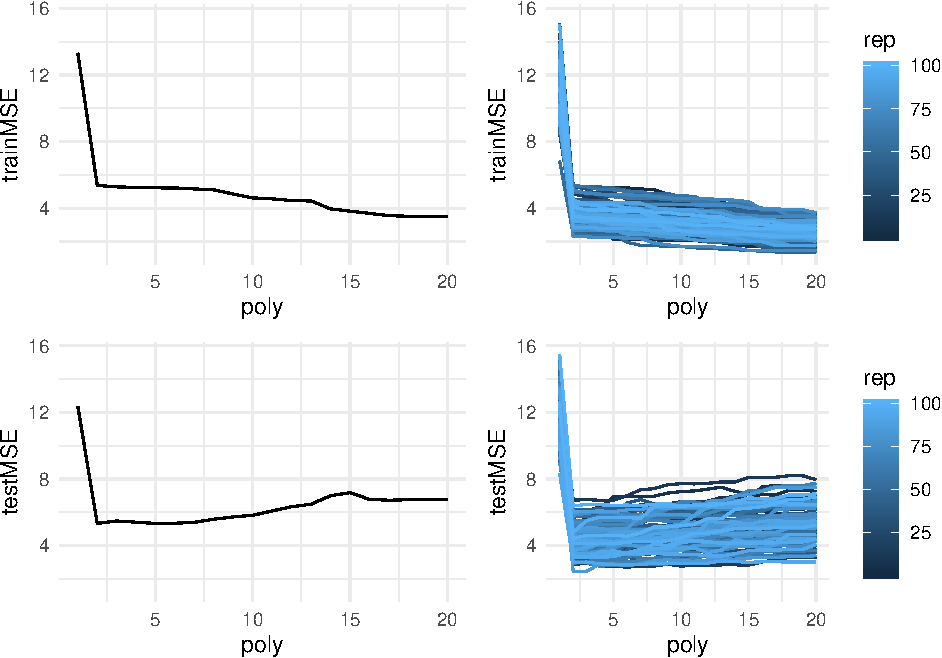
\includegraphics{4Classif_files/figure-beamer/unnamed-chunk-13-1.pdf}

\end{frame}

\begin{frame}[fragile]

The above plots shows \texttt{default} as a function of \texttt{balance}
and \texttt{default} as a function of \texttt{income} with corresponding
fitted linear regression lines (red for \texttt{x=balance} and orange
for \texttt{x=income}). Notice that linear regression in this case
produces predictions that are smaller than zero or bigger than one, this
it is hard to interpret these as probabilities.

It is still possible to use linear regression for classification
problems with two classes. It turns out that - if the conditional class
densities are (multivariate) normal with equal covariance matrices then
this linear regression (with 0 and 1 response) will in fact give the
same classification as LDA. See e.g.~Ripley (1995), Section 3.2.

\end{frame}

\begin{frame}

\textbf{Using linear regression on a classification problem?}

\textbf{Example 2: } Suppose we want to classify a film. We have defined
three classes: \{ drama, comedy, science-fiction\}. We could try to
model this using linear regression and the following coding:
\[Y = \begin{cases} 1 \quad \text{if drama}, \\ 2 \quad \text{if comedy}, \\ 3 \quad \text{if science-fiction}.\end{cases}\]
However, this coding implies an ordering of the variables and that the
difference between the classes is equal. There is in general no natural
way to code a quantitative variable with more than two classes such that
it can be used with linear regression.

\end{frame}

\begin{frame}

So, using linear regression to solve a classification problem seems hard
with more than two classes - as done here. But, it turns out that using
a dummy variable conding for the classes, it is possible to produce the
same result as LDA (also with many classes). This is the starting point
for \emph{flexible discriminant analysis}.

Linear regression to do classification is not a bad idea, but requires
some extra work (multivariate Y due to the dummy variable coding).
Therefore we leave linear regression for now.

For two classes \emph{binary regression}, in particular \emph{logistic
regression}, is very popular - and is up next.

\end{frame}

\begin{frame}{Logistic regression}

In logistic regression we consider a classification problem with two
classes.

\begin{block}{The model}

Assume that \(Y\) is coded (\(\mathcal{C} = \{1, 0\}\) or \{success,
failure\}), and we focus on success. We may assume that \(Y_i\) follows
a Bernoulli distribution with probability of success \(p_i\).

\[Y_i = \begin{cases} 1 \text{ with probability } p_i, \\ 0 \text{ with probability } 1-p_i. \end{cases}\]

In logistic regression we \emph{link} together our covariates
\({\bf x}_i\) with this probability \(p_i\) using a \emph{logistic
function}.

\end{block}

\end{frame}

\begin{frame}

In the case of one covariate, the logistic function has the form:
\[ p_i= \frac{e^{\beta_0+\beta_1 x_i}}{1 + e^{\beta_0 + \beta_1 x_i}}.\]

This function is S-shaped, and ranges between 0 and 1 (so the \(p_i\) is
between 0 and 1). The parameter \(\beta_1\) determines the rate of
increase or decrease of the S-shaped curve, and the sign indicates
whether the curve ascends or descends.

\textbf{Q:} Where did that come from? There are other transforms that
takes a linear predictor and transforms into the range 0 to 1.

\end{frame}

\begin{frame}[fragile]

Logistic regression ensures that the estimated probabilities lie in the
interval between 0 and 1. This is illustrated in the figure below. The
blue line shows the fitted line when performing logistic regression on
\texttt{default} as a function of \texttt{balance}.

The parameters are estimated using the method of maximum likelihood - we
will look at that soon, but first we look at how to interpret the
estimated parameters.

\end{frame}

\begin{frame}

\begin{block}{Example estimated \(\beta\) and logistic curve}

\includegraphics{4Classif_files/figure-beamer/defaultglm-1.pdf}

Default data: here \(\hat{\beta}_0=\) -10.65 and \(\hat{\beta}_1=\)
0.005.

\end{block}

\end{frame}

\begin{frame}[fragile]

Observe effect of intercept and slope term:

\[p_i= \frac{e^{\beta_0+\beta_1 x_i}}{1 + e^{\beta_0 + \beta_1 x_i}}\]

Solid lines: \(\beta_0=0\) and \(\beta_1\) is \(0.8\) (blue), \(1\)
(red) and \(2\) (orange). Dashed lines \(\beta_0=1\).

\begin{Shaded}
\begin{Highlighting}[]
\KeywordTok{library}\NormalTok{(ggplot2)}
\KeywordTok{ggplot}\NormalTok{(}\KeywordTok{data.frame}\NormalTok{(}\DataTypeTok{x =} \KeywordTok{c}\NormalTok{(}\OperatorTok{-}\DecValTok{6}\NormalTok{, }\DecValTok{5}\NormalTok{)), }\KeywordTok{aes}\NormalTok{(x)) }\OperatorTok{+}\StringTok{ }\KeywordTok{xlab}\NormalTok{(}\KeywordTok{expression}\NormalTok{(x)) }\OperatorTok{+}\StringTok{ }\KeywordTok{ylab}\NormalTok{(}\KeywordTok{expression}\NormalTok{(mu)) }\OperatorTok{+}\StringTok{ }
\StringTok{    }\KeywordTok{stat_function}\NormalTok{(}\DataTypeTok{fun =} \ControlFlowTok{function}\NormalTok{(x) }\KeywordTok{exp}\NormalTok{(x)}\OperatorTok{/}\NormalTok{(}\DecValTok{1} \OperatorTok{+}\StringTok{ }\KeywordTok{exp}\NormalTok{(x)), }\DataTypeTok{geom =} \StringTok{"line"}\NormalTok{, }
        \DataTypeTok{colour =} \StringTok{"red"}\NormalTok{) }\OperatorTok{+}\StringTok{ }\KeywordTok{stat_function}\NormalTok{(}\DataTypeTok{fun =} \ControlFlowTok{function}\NormalTok{(x) }\KeywordTok{exp}\NormalTok{(}\DecValTok{2} \OperatorTok{*}\StringTok{ }\NormalTok{x)}\OperatorTok{/}\NormalTok{(}\DecValTok{1} \OperatorTok{+}\StringTok{ }
\StringTok{    }\KeywordTok{exp}\NormalTok{(}\DecValTok{2} \OperatorTok{*}\StringTok{ }\NormalTok{x)), }\DataTypeTok{geom =} \StringTok{"line"}\NormalTok{, }\DataTypeTok{colour =} \StringTok{"orange"}\NormalTok{) }\OperatorTok{+}\StringTok{ }\KeywordTok{stat_function}\NormalTok{(}\DataTypeTok{fun =} \ControlFlowTok{function}\NormalTok{(x) }\KeywordTok{exp}\NormalTok{(}\FloatTok{0.8} \OperatorTok{*}\StringTok{ }
\StringTok{    }\NormalTok{x)}\OperatorTok{/}\NormalTok{(}\DecValTok{1} \OperatorTok{+}\StringTok{ }\KeywordTok{exp}\NormalTok{(}\FloatTok{0.8} \OperatorTok{*}\StringTok{ }\NormalTok{x)), }\DataTypeTok{geom =} \StringTok{"line"}\NormalTok{, }\DataTypeTok{colour =} \StringTok{"blue"}\NormalTok{) }\OperatorTok{+}\StringTok{ }\KeywordTok{stat_function}\NormalTok{(}\DataTypeTok{fun =} \ControlFlowTok{function}\NormalTok{(x) }\KeywordTok{exp}\NormalTok{(}\DecValTok{1} \OperatorTok{+}\StringTok{ }
\StringTok{    }\NormalTok{x)}\OperatorTok{/}\NormalTok{(}\DecValTok{1} \OperatorTok{+}\StringTok{ }\KeywordTok{exp}\NormalTok{(}\DecValTok{1} \OperatorTok{+}\StringTok{ }\NormalTok{x)), }\DataTypeTok{geom =} \StringTok{"line"}\NormalTok{, }\DataTypeTok{colour =} \StringTok{"red"}\NormalTok{, }\DataTypeTok{linetype =} \StringTok{"dashed"}\NormalTok{) }\OperatorTok{+}\StringTok{ }
\StringTok{    }\KeywordTok{stat_function}\NormalTok{(}\DataTypeTok{fun =} \ControlFlowTok{function}\NormalTok{(x) }\KeywordTok{exp}\NormalTok{(}\DecValTok{1} \OperatorTok{+}\StringTok{ }\DecValTok{2} \OperatorTok{*}\StringTok{ }\NormalTok{x)}\OperatorTok{/}\NormalTok{(}\DecValTok{1} \OperatorTok{+}\StringTok{ }\KeywordTok{exp}\NormalTok{(}\DecValTok{1} \OperatorTok{+}\StringTok{ }\DecValTok{2} \OperatorTok{*}\StringTok{ }\NormalTok{x)), }
        \DataTypeTok{geom =} \StringTok{"line"}\NormalTok{, }\DataTypeTok{colour =} \StringTok{"orange"}\NormalTok{, }\DataTypeTok{linetype =} \StringTok{"dashed"}\NormalTok{) }\OperatorTok{+}\StringTok{ }\KeywordTok{stat_function}\NormalTok{(}\DataTypeTok{fun =} \ControlFlowTok{function}\NormalTok{(x) }\KeywordTok{exp}\NormalTok{(}\DecValTok{1} \OperatorTok{+}\StringTok{ }
\StringTok{    }\FloatTok{0.8} \OperatorTok{*}\StringTok{ }\NormalTok{x)}\OperatorTok{/}\NormalTok{(}\DecValTok{1} \OperatorTok{+}\StringTok{ }\KeywordTok{exp}\NormalTok{(}\DecValTok{1} \OperatorTok{+}\StringTok{ }\FloatTok{0.8} \OperatorTok{*}\StringTok{ }\NormalTok{x)), }\DataTypeTok{geom =} \StringTok{"line"}\NormalTok{, }\DataTypeTok{colour =} \StringTok{"blue"}\NormalTok{, }
    \DataTypeTok{linetype =} \StringTok{"dashed"}\NormalTok{) }\OperatorTok{+}\StringTok{ }\KeywordTok{scale_colour_manual}\NormalTok{(}\StringTok{"0+k x"}\NormalTok{, }\DataTypeTok{values =} \KeywordTok{c}\NormalTok{(}\StringTok{"red"}\NormalTok{, }
    \StringTok{"orange"}\NormalTok{, }\StringTok{"blue"}\NormalTok{), }\DataTypeTok{labels =} \KeywordTok{c}\NormalTok{(}\StringTok{"1"}\NormalTok{, }\StringTok{"2"}\NormalTok{, }\StringTok{"0.8"}\NormalTok{))}
\end{Highlighting}
\end{Shaded}

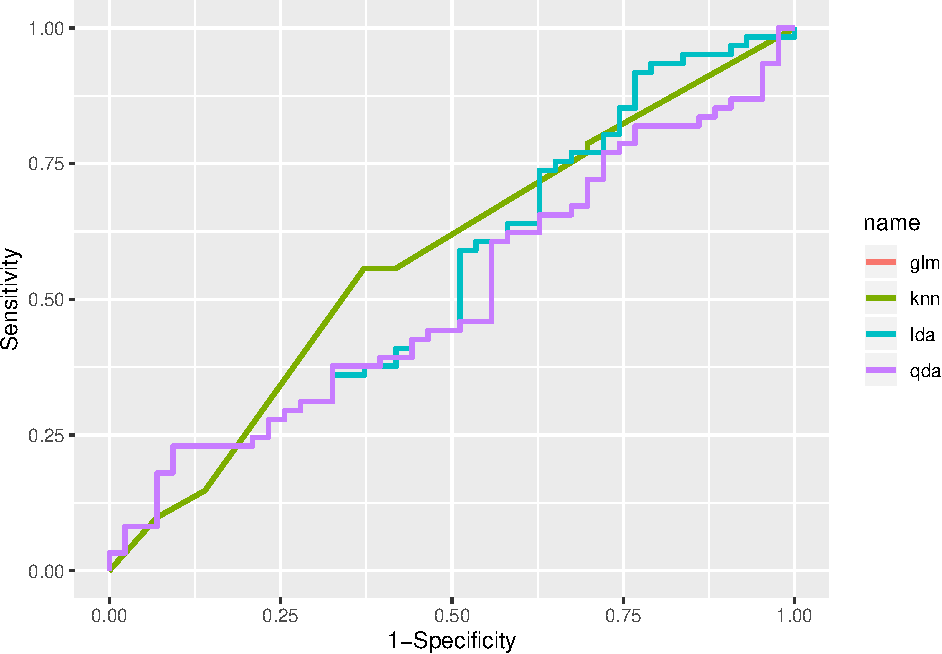
\includegraphics{4Classif_files/figure-beamer/unnamed-chunk-14-1.pdf}

\end{frame}

\begin{frame}[fragile]

\begin{block}{The odds and the odds ratio}

For the logistic regression it is hard to give a simple interpretation
regression coefficients \(\beta\), because an increase in \(x_1\) by one
unit does not give the same increase (decrease) in the probability
\(p_i\) for all values of \(x_1\). But, looking at odds - it is simpler
to explain what the \(\beta\)s mean.

For a probability \(p_i\) the ratio \(\frac{p_i}{1-p_1}\) is called the
\emph{odds}.

If \(p_i=\frac{1}{2}\) then the odds is \(1\), and if
\(p_i=\frac{1}{4}\) then the odds is \(\frac{1}{3}\). We may make a
table for probability vs.~odds in R:

\begin{Shaded}
\begin{Highlighting}[]
\KeywordTok{library}\NormalTok{(knitr)}
\KeywordTok{library}\NormalTok{(kableExtra)}
\NormalTok{p =}\StringTok{ }\KeywordTok{seq}\NormalTok{(}\FloatTok{0.1}\NormalTok{, }\FloatTok{0.9}\NormalTok{, }\FloatTok{0.1}\NormalTok{)}
\NormalTok{odds =}\StringTok{ }\NormalTok{p}\OperatorTok{/}\NormalTok{(}\DecValTok{1} \OperatorTok{-}\StringTok{ }\NormalTok{p)}
\KeywordTok{kable}\NormalTok{(}\KeywordTok{t}\NormalTok{(}\KeywordTok{data.frame}\NormalTok{(p, odds)), }\DataTypeTok{digits =} \KeywordTok{c}\NormalTok{(}\DecValTok{2}\NormalTok{, }\DecValTok{2}\NormalTok{), }\DataTypeTok{format =}\NormalTok{ whichformat)}
\end{Highlighting}
\end{Shaded}

p

0.10

0.20

0.30

0.40

0.5

0.6

0.70

0.8

0.9

odds

0.11

0.25

0.43

0.67

1.0

1.5

2.33

4.0

9.0

Odds may be seen to be a better scale than probability to represent
chance, and is used in betting. In addition, odds are unbounded above.

\end{block}

\end{frame}

\begin{frame}

\textbf{Why is the odds relevant?}

(Since \(p\) is used for probability we use \(r\) for number of
covariates now.)

Let us assume that we have \(r\) covariates, and we use \(\eta_i\)
(linear predictor) to help with our notation.

\begin{align*}
\eta_i&= \beta_0+\beta_1 x_{i1}+\beta_2 x_{i2}+\cdots + \beta_r x_{ir}\\
p_i&= \frac{\exp(\eta_i)}{1+\exp(\eta_i)}\\
\eta_i&=\ln(\frac{p_i}{1-p_i})\\
\ln(\frac{p_i}{1-p_i})&=\beta_0+\beta_1 x_{i1}+\beta_2 x_{i2}+\cdots + \beta_r x_{ir}\\
\frac{p_i}{1-p_i}=&\frac{P(Y_i=1|{\bf x}_i)}{P(Y_i=0|{\bf x}_i)}=\exp(\beta_0)\cdot \exp(\beta_1 x_{i1})\cdots\exp(\beta_r x_{ir})
\end{align*}

We have a \emph{multiplicative model} for the odds - which can help us
to interpret our \(\beta\)s.

In addition we see that the \emph{logit} of \(p_i\),
\(\ln(\frac{p_i}{1-p_i})\), is linear in the \(\beta\)s (and in the
\(x\)'s).

\end{frame}

\begin{frame}

\textbf{So, what if we increase \(x_{1i}\) to \(x_{1i}+1\)?}

If the covariate \(x_{1i}\) increases by one unit (while all other
covariates are kept fixed) then the odds is multiplied by
\(\exp(\beta_1)\):

\begin{align*}
\frac{P(Y_i=1\mid x_{i1}+1)}{P(Y_i=0)\mid x_{i1}+1)}&=\exp(\beta_0)\cdot \exp(\beta_1 (x_{i1}+1))\exp(\beta_2 (x_{i2}))\cdots\exp(\beta_r x_{ir})\\
&=\exp(\beta_0)\cdot \exp(\beta_1 x_{i1})\exp(\beta_1)\exp(\beta_2 x_{i2})\cdots\exp(\beta_r x_{ir})\\
&=\frac{P(Y_i=1\mid x_{i1})}{P(Y_i=0\mid x_{i1})}\cdot \exp(\beta_1)\\
\end{align*}

This means that if \(x_{i1}\) increases by \(1\) then: if \(\beta_1<0\)
we get a decrease in the odds, if \(\beta_1=0\) no change, and if
\(\beta_1>0\) we have an increase. Here \(\exp(\beta_1)\) is easier to
interpret than \(\beta_1\).

\end{frame}

\begin{frame}[fragile]

\begin{block}{Default-example}

Default as response and student, balance and income as covariates

Result:
\[\frac{P(Y_i=1\mid x_{i1}+1)}{P(Y_i=0)\mid x_{i1}+1)}=\frac{P(Y_i=1\mid x_{i1})}{P(Y_i=0\mid x_{i1})}\cdot \exp(\beta_1)\]

What is done below? Explain what the effect of \texttt{student} gives.

\footnotesize

\begin{Shaded}
\begin{Highlighting}[]
\KeywordTok{colnames}\NormalTok{(Default)}
\NormalTok{fit =}\StringTok{ }\KeywordTok{glm}\NormalTok{(default }\OperatorTok{~}\StringTok{ }\NormalTok{student }\OperatorTok{+}\StringTok{ }\NormalTok{balance }\OperatorTok{+}\StringTok{ }\NormalTok{income, }\DataTypeTok{family =} \StringTok{"binomial"}\NormalTok{, }
    \DataTypeTok{data =}\NormalTok{ Default)}
\KeywordTok{coef}\NormalTok{(fit)}
\KeywordTok{round}\NormalTok{(}\KeywordTok{exp}\NormalTok{(}\KeywordTok{coef}\NormalTok{(fit)), }\DecValTok{3}\NormalTok{)}
\end{Highlighting}
\end{Shaded}

\begin{verbatim}
## [1] "default" "student" "balance" "income" 
##   (Intercept)    studentYes       balance        income 
## -1.086905e+01 -6.467758e-01  5.736505e-03  3.033450e-06 
## (Intercept)  studentYes     balance      income 
##       0.000       0.524       1.006       1.000
\end{verbatim}

\normalsize

\end{block}

\end{frame}

\begin{frame}

\begin{block}{Maximum likelihood estimation}

We assume that pairs of covariates and responses \(\{x_i, y_i\}\) are
measured independently of each other. Given \(n\) such observation
pairs, the likelihood function of a logistic regression model can be
written as:
\[L(\boldsymbol{\beta}) = \prod_{i=1}^n L_i(\boldsymbol{\beta}) = \prod_{i=1}^n f(y_i; \boldsymbol{\beta}) = \prod_{i=1}^n (p_i)^{y_i}(1-p_i)^{1-y_i},\]
where
\(\boldsymbol{\beta} = (\beta_0, \beta_1, \beta_2, \ldots, \beta_r)^T\)
enters into \(p_i\).

\[p_i= \frac{\exp(\beta_0+\beta_1 x_{i1}+\cdots + \beta_p x_{ir})}{1 + \exp(\beta_0 + \beta_1 x_{i1}+\cdots+\beta_r x_{ir})}\]

\end{block}

\end{frame}

\begin{frame}

The maximum likelihood estimates are found by maximizing the likelihood,
and since the log is a monotone transform (and maximizing the
log-likelihood will give the same result as maximizing the likelihood)
we usually work with the log-likelihood (because this makes the maths
easier).

\begin{align*} \ln(L(\boldsymbol{\beta}))&=l(\boldsymbol{\beta}) =\sum_{i=1}^n \Big ( y_i \log p_i + (1-y_i) \log(1 - p_i )\Big ) \\ &= \sum_{i=1}^n \Big ( y_i \log \Big (\frac{p_i}{1-p_i} \Big) + \log(1-p_i) \Big ) \\
&= \sum_{i=1}^n \Big (y_i (\beta_0 + \beta_1 x_{i1}+\cdots + \beta_r x_{ir}) - \log(1 + e^{\beta_0 + \beta_1 x_{i1}+\cdots + \beta_p x_{ir}} \Big ).\end{align*}

\end{frame}

\begin{frame}

\begin{itemize}
\tightlist
\item
  To maximize the log-likelihood function we find the \(r+1\) partial
  derivatives, and set equal til 0.
\item
  This gives us a set of \(r+1\) non-linear equations in the \(\beta\)s.
\item
  This set of equations does not have a closed form solution.
\item
  These equations are therefore solved numerically. The
  \emph{Newton-Raphson algorithm} (or Fisher Scoring) is used.
\end{itemize}

\end{frame}

\begin{frame}[fragile]

\footnotesize

\begin{Shaded}
\begin{Highlighting}[]
\NormalTok{fit =}\StringTok{ }\KeywordTok{glm}\NormalTok{(default }\OperatorTok{~}\StringTok{ }\NormalTok{student }\OperatorTok{+}\StringTok{ }\NormalTok{balance }\OperatorTok{+}\StringTok{ }\NormalTok{income, }\DataTypeTok{family =} \StringTok{"binomial"}\NormalTok{, }
    \DataTypeTok{data =}\NormalTok{ Default)}
\KeywordTok{summary}\NormalTok{(fit)}
\end{Highlighting}
\end{Shaded}

\begin{verbatim}
## 
## Call:
## glm(formula = default ~ student + balance + income, family = "binomial", 
##     data = Default)
## 
## Deviance Residuals: 
##     Min       1Q   Median       3Q      Max  
## -2.4691  -0.1418  -0.0557  -0.0203   3.7383  
## 
## Coefficients:
##               Estimate Std. Error z value Pr(>|z|)    
## (Intercept) -1.087e+01  4.923e-01 -22.080  < 2e-16 ***
## studentYes  -6.468e-01  2.363e-01  -2.738  0.00619 ** 
## balance      5.737e-03  2.319e-04  24.738  < 2e-16 ***
## income       3.033e-06  8.203e-06   0.370  0.71152    
## ---
## Signif. codes:  0 '***' 0.001 '**' 0.01 '*' 0.05 '.' 0.1 ' ' 1
## 
## (Dispersion parameter for binomial family taken to be 1)
## 
##     Null deviance: 2920.6  on 9999  degrees of freedom
## Residual deviance: 1571.5  on 9996  degrees of freedom
## AIC: 1579.5
## 
## Number of Fisher Scoring iterations: 8
\end{verbatim}

\normalsize

\end{frame}

\begin{frame}

\begin{block}{Inference}

We may construct confidence intervals and test hypotheses about the
\(\beta\)s, with the aim to understand which covariate that contributes
to our posterior probabilites and classification.

This is done by assuming that each \(\hat{\beta}_j\) is approximately
normally distributed with mean \(\beta_j\) and variance
\(\hat{\text{Var}}(\hat{\beta}_j)\) (related to the negative of the
inverse of the expected Hessian of the loglikelihood function).

\end{block}

\end{frame}

\begin{frame}

\begin{block}{The Akaike Information Criterion (AIC) for model
selection}

The AIC score is given by:
\[AIC = 2 \cdot (r+1) -2 \cdot \text{loglik},\] where \(r+1\) is the
number of model parameters. The loglik is the maximized log-likelihood
\(l(\hat{\boldsymbol{\beta}})\) and \(\hat{\boldsymbol{\beta}}\) is the
maximum-likelihood estimate of the parameter-vector
\(\boldsymbol{\beta} = (\beta_0, \beta_1, ..., \beta_{r})^T\). The role
of \(r+1\) is to penalize models with many parameters as a high number
of parameters may lead to overfitting. The AIC value can be used to
choose between candidate logistic regression models, where the model
with the lowest AIC value is the one expected to give the best fit.

More about the AIC in Module 6.

\end{block}

\end{frame}

\begin{frame}

\begin{block}{Predictions}

\begin{itemize}
\tightlist
\item
  We fit a (simple) logistic regression model to our data set, and
\item
  get parameter estimates \(\hat{\beta}_0\) and \(\hat{\beta}_1\).
\item
  We want to use this model to make a prediction when given a new
  observation \(x_0\).
\end{itemize}

\[\hat{p}(x_0) = \frac{e^{\hat{\beta}_0 + \hat{\beta}_1 x_0}}{1+e^{\hat{\beta}_0 + \hat{\beta}_1 x_0}} \]

This \(\hat{p}(x_0)\) is the estimated probability that the new
observation \(x_0\) belongs to the class defined by \(Y=1\).

In the case of qualitative covariates, a dummy variable needs to be
introduced. This is done in a similar fashion as for linear regression.

\end{block}

\end{frame}

\begin{frame}

\begin{block}{Want to learn more (theory) about logistic regression?}

In TMA4315 Generalized linear models we spent 3 weeks with binary
regression - mainly logistic regression. The focus there was on all
parts of the regression (not classification) with a mathematical focus
on estimation, inference, model fit.

\end{block}

\end{frame}

\begin{frame}[fragile]

\begin{block}{Example: South African heart disease data set}

In this example we use the \texttt{SAhert} data set from the
\texttt{ElemStatLearn} package. This is a retrospective sample of males
in a heart-disease high-risk region in South Africa. It consists of 462
observations on the 10 variables. All subjects are male in the age range
15-64. There are 160 cases (individuals who have suffered from a
conorary heart disease) and 302 controls (individuals who have not
suffered from a conorary heart disease).

\end{block}

\end{frame}

\begin{frame}[fragile]

The response value (\texttt{chd}) and covariates

\begin{itemize}
\tightlist
\item
  \texttt{chd} : conorary heart disease \{yes, no\} coded by the numbers
  \{1, 0\}
\item
  \texttt{sbp} : systolic blood pressure\\
\item
  \texttt{tobacco} : cumulative tobacco (kg)\\
\item
  \texttt{ldl} : low density lipoprotein cholesterol
\item
  \texttt{adiposity} : a numeric vector
\item
  \texttt{famhist} : family history of heart disease. Categorical
  variable with two levels: \{Absent, Present\}.
\item
  \texttt{typea} : type-A behavior
\item
  \texttt{obesity} : a numerical value
\item
  \texttt{alcohol} : current alcohol consumption
\item
  \texttt{age} : age at onset
\end{itemize}

The goal is to identify important risk factors. We start by loading and
looking at the data:

\end{frame}

\begin{frame}[fragile]

\footnotesize

\begin{Shaded}
\begin{Highlighting}[]
\KeywordTok{library}\NormalTok{(ElemStatLearn)}
\KeywordTok{library}\NormalTok{(knitr)}
\KeywordTok{library}\NormalTok{(kableExtra)}
\NormalTok{heartds =}\StringTok{ }\NormalTok{SAheart}
\NormalTok{heartds}\OperatorTok{$}\NormalTok{chd =}\StringTok{ }\KeywordTok{as.factor}\NormalTok{(heartds}\OperatorTok{$}\NormalTok{chd)}
\KeywordTok{kable}\NormalTok{(}\KeywordTok{head}\NormalTok{(heartds), }\DataTypeTok{format =}\NormalTok{ whichformat)}
\end{Highlighting}
\end{Shaded}

sbp

tobacco

ldl

adiposity

famhist

typea

obesity

alcohol

age

chd

160

12.00

5.73

23.11

Present

49

25.30

97.20

52

1

144

0.01

4.41

28.61

Absent

55

28.87

2.06

63

1

118

0.08

3.48

32.28

Present

52

29.14

3.81

46

0

170

7.50

6.41

38.03

Present

51

31.99

24.26

58

1

134

13.60

3.50

27.78

Present

60

25.99

57.34

49

1

132

6.20

6.47

36.21

Present

62

30.77

14.14

45

0

\normalsize

\end{frame}

\begin{frame}[fragile]

In order to investigate the data further, we use the \texttt{ggpairs}
function from the \texttt{GGally} library, to make scatter plots of the
covariates. The coloring is done according to the response variable,
where green represents a case \(Y=1\) and red represents a control
\(Y=0\).

\end{frame}

\begin{frame}[fragile]

\begin{Shaded}
\begin{Highlighting}[]
\KeywordTok{library}\NormalTok{(ggplot2)}
\KeywordTok{library}\NormalTok{(GGally)}
\KeywordTok{ggpairs}\NormalTok{(heartds, ggplot2}\OperatorTok{::}\KeywordTok{aes}\NormalTok{(}\DataTypeTok{color=}\NormalTok{chd), }\CommentTok{#upper="blank",  }
        \DataTypeTok{lower =} \KeywordTok{list}\NormalTok{(}\DataTypeTok{continuous =} \KeywordTok{wrap}\NormalTok{(}\StringTok{"points"}\NormalTok{, }\DataTypeTok{alpha =} \FloatTok{0.3}\NormalTok{, }\DataTypeTok{size=}\FloatTok{0.2}\NormalTok{)))}
\end{Highlighting}
\end{Shaded}

\end{frame}

\begin{frame}[fragile]

We now fit a (multiple) logistic regression model using the \texttt{glm}
function and the full data set. In order to fit a logistic model, the
\texttt{family} argument must be set equal to \texttt{="binomial"}. The
\texttt{summary} function prints out the estimates of the coefficients,
their standard errors and z-values. As for a linear regression model,
the significant coefficients are indicated by stars where the
significant codes are included in the \texttt{R} outprint.

\end{frame}

\begin{frame}[fragile]

\footnotesize

\begin{Shaded}
\begin{Highlighting}[]
\NormalTok{glm_heart =}\StringTok{ }\KeywordTok{glm}\NormalTok{(chd }\OperatorTok{~}\StringTok{ }\NormalTok{., }\DataTypeTok{data =}\NormalTok{ heartds, }\DataTypeTok{family =} \StringTok{"binomial"}\NormalTok{)}
\KeywordTok{summary}\NormalTok{(glm_heart)}
\end{Highlighting}
\end{Shaded}

\begin{verbatim}
## 
## Call:
## glm(formula = chd ~ ., family = "binomial", data = heartds)
## 
## Deviance Residuals: 
##     Min       1Q   Median       3Q      Max  
## -1.7781  -0.8213  -0.4387   0.8889   2.5435  
## 
## Coefficients:
##                  Estimate Std. Error z value Pr(>|z|)    
## (Intercept)    -6.1507209  1.3082600  -4.701 2.58e-06 ***
## sbp             0.0065040  0.0057304   1.135 0.256374    
## tobacco         0.0793764  0.0266028   2.984 0.002847 ** 
## ldl             0.1739239  0.0596617   2.915 0.003555 ** 
## adiposity       0.0185866  0.0292894   0.635 0.525700    
## famhistPresent  0.9253704  0.2278940   4.061 4.90e-05 ***
## typea           0.0395950  0.0123202   3.214 0.001310 ** 
## obesity        -0.0629099  0.0442477  -1.422 0.155095    
## alcohol         0.0001217  0.0044832   0.027 0.978350    
## age             0.0452253  0.0121298   3.728 0.000193 ***
## ---
## Signif. codes:  0 '***' 0.001 '**' 0.01 '*' 0.05 '.' 0.1 ' ' 1
## 
## (Dispersion parameter for binomial family taken to be 1)
## 
##     Null deviance: 596.11  on 461  degrees of freedom
## Residual deviance: 472.14  on 452  degrees of freedom
## AIC: 492.14
## 
## Number of Fisher Scoring iterations: 5
\end{verbatim}

\normalsize

\end{frame}

\begin{frame}

Estimated coeffs

exp(estimated coeffs)

(Intercept)

-6.151

0.002

sbp

0.007

1.007

tobacco

0.079

1.083

ldl

0.174

1.190

adiposity

0.019

1.019

famhistPresent

0.925

2.523

typea

0.040

1.040

obesity

-0.063

0.939

alcohol

0.000

1.000

age

0.045

1.046

How did we find the coefficients and what does the second column mean?

\end{frame}

\begin{frame}[fragile]

\begin{block}{Multinomial logistic regression}

The logistic regression model can be generalized for a response variable
with more than two classes. Assume we have a response variable with
\(K\) possible classes and \(r\) covariates. The probability that \(Y\)
belongs to class \(k\), given an observation vector
\(\mathbf{x} = (x_1, x_2, \dots, x_r)^T\) is (usually) modelled by:

\[\ln \frac{P(Y = k | \mathbf{x})}{P(Y = K | \mathbf{x})}= \beta_{0k} + \beta_{1k} x_1 + \cdots + \beta_{rk} x_r.\]

The multinomial logistic regression model is implemented in the
\texttt{glmnet} or \texttt{VGAM} package in \texttt{R}.

We will not discuss this further since LDA is more popular (than
logistic regression) in the multi-class setting. And, as we shall see
soon - they are not that different.

\end{block}

\end{frame}

\begin{frame}{Confusion matrix, sensitivity, specificity}

In a two class problem - assume the classes are labelled ``-'' (non
disease) and ``+'' (disease). In a population setting we define the
following event and associated number of observations.

Predicted -

Predicted +

Total

True -

True Negative TN

False Positive FP

N

True +

False Negative FN

True Positive TP

P

Total

N*

P*

\end{frame}

\begin{frame}

\textbf{Sensitivity} is the proportion of correctly classified positive
observations:
\(\frac{\# \text{True Positive}}{\# \text{Condition Positive}}=\frac{\text{TP}}{\text{P}}\).

\textbf{Specificity} is the proportion of correctly classified negative
observations:
\(\frac{\# \text{True Negative}}{\# \text{Condition Negative}}=\frac{\text{TN}}{\text{N}}\).

We would like that a classification rule (or a diagnostic test) have
both a high sensitivity and a high specificity.

\end{frame}

\begin{frame}

Other useful quantities:

Name

Definition

Synonyms

False positive rate

FP/N

Type I error, 1-specificity

True positive rate

TP/P

1-Type II error, power, sensitivity, recall

Positive predictive value (PPV)

TP/P*

Precision, 1-false discovery proportion

Negative predictive value (NPV)

TN/N*

(These two tables are tables 4.6 and 4.7 in our ISL-textbook.)

\end{frame}

\begin{frame}[fragile]

\begin{block}{Example Continued: South African heart disease}

We want to evaluate our multiple logistic model for the \texttt{SAheart}
data set. In order to investigate the training error and the test error,
we divide the original data set, randomly, into two samples of equal
size.

\begin{Shaded}
\begin{Highlighting}[]
\KeywordTok{set.seed}\NormalTok{(}\DecValTok{20}\NormalTok{)}
\NormalTok{train_ID =}\StringTok{ }\KeywordTok{sample}\NormalTok{(}\DecValTok{1}\OperatorTok{:}\KeywordTok{nrow}\NormalTok{(heartds), }\KeywordTok{nrow}\NormalTok{(heartds)}\OperatorTok{/}\DecValTok{2}\NormalTok{)}
\NormalTok{train_SA =}\StringTok{ }\NormalTok{heartds[train_ID, ]}
\NormalTok{test_SA =}\StringTok{ }\NormalTok{heartds[}\OperatorTok{-}\NormalTok{train_ID, ]}
\end{Highlighting}
\end{Shaded}

\end{block}

\end{frame}

\begin{frame}[fragile]

We now fit a logistic regression model, using the training set only:

\footnotesize

\begin{Shaded}
\begin{Highlighting}[]
\NormalTok{glm_SA =}\StringTok{ }\KeywordTok{glm}\NormalTok{(chd }\OperatorTok{~}\StringTok{ }\NormalTok{., }\DataTypeTok{data =}\NormalTok{ train_SA, }\DataTypeTok{family =} \StringTok{"binomial"}\NormalTok{)}
\KeywordTok{summary}\NormalTok{(glm_SA)}
\end{Highlighting}
\end{Shaded}

\begin{verbatim}
## 
## Call:
## glm(formula = chd ~ ., family = "binomial", data = train_SA)
## 
## Deviance Residuals: 
##     Min       1Q   Median       3Q      Max  
## -2.0583  -0.7660  -0.4523   0.8679   2.2682  
## 
## Coefficients:
##                  Estimate Std. Error z value Pr(>|z|)   
## (Intercept)    -5.4999981  1.9010122  -2.893  0.00381 **
## sbp             0.0050738  0.0089677   0.566  0.57154   
## tobacco         0.1228036  0.0443098   2.771  0.00558 **
## ldl             0.0315840  0.0817017   0.387  0.69907   
## adiposity       0.0223541  0.0398203   0.561  0.57454   
## famhistPresent  0.7763880  0.3434487   2.261  0.02379 * 
## typea           0.0328267  0.0181739   1.806  0.07088 . 
## obesity        -0.0487256  0.0592647  -0.822  0.41098   
## alcohol        -0.0007868  0.0079569  -0.099  0.92123   
## age             0.0470105  0.0170190   2.762  0.00574 **
## ---
## Signif. codes:  0 '***' 0.001 '**' 0.01 '*' 0.05 '.' 0.1 ' ' 1
## 
## (Dispersion parameter for binomial family taken to be 1)
## 
##     Null deviance: 289.73  on 230  degrees of freedom
## Residual deviance: 229.18  on 221  degrees of freedom
## AIC: 249.18
## 
## Number of Fisher Scoring iterations: 5
\end{verbatim}

\normalsize

\end{frame}

\begin{frame}[fragile]

By comparing this outprint with the corresponding outprint above, we see
that the estimated coefficients slightly differ. This is because a
different data set has been used to fit the model. We previously used
the full data set.

We want to estimate the probability of a \texttt{chd} event for the
observations in the test set. To do this we can insert the estimated
coefficient into the logistic equation, remembering that
\texttt{famhist} is a categorical covariate, modeled by a dummy
variable:
\[x_\text{famhist} = \begin{cases} 1, \quad \text{ if Present}, \\ 0, \quad \text{ if Absent}.\end{cases}\]
The estimated probability of \(Y=1\) if \texttt{famhist\ =\ "Present"},
given a vector \(\mathbf{X}\) of covariate observations is:
\[\hat{p}(\mathbf{X}) =\frac{e^{-7.43 + 0.01 x_{\text{sbp}} + 0.09 x_{\text{tobacco}} + 0.16 x_\text{ldh} + 0.01 x_\text{adiposity}+1.04 \cdot 1 + 0.04 x_\text{typea}-0.04 x_\text{obesity}-0.005 x_\text{alcohol} +0.05 x_{\text{age}}}}{1+e^{-7.43 + 0.01 x_{\text{sbp}} + 0.09 x_{\text{tobacco}} + 0.16 x_\text{ldh} + 0.01 x_\text{adiposity}+1.04 \cdot 1 + 0.04 x_\text{typea}-0.04 x_\text{obesity}-0.005 x_\text{alcohol} +0.05 x_{\text{age}}}} .\]
Whereas, if \texttt{famhist\ =\ "Absent"} the estimated probability is:
\[\hat{p}(\mathbf{X}) =\frac{e^{-7.43 + 0.01 x_{\text{sbp}} + 0.09 x_{\text{tobacco}} + 0.16 x_\text{ldh} + 0.01 x_\text{adiposity}+1.04 \cdot 0 + 0.04 x_\text{typea}-0.04 x_\text{obesity}-0.005 x_\text{alcohol} +0.05 x_{\text{age}}}}{1+e^{-7.43 + 0.01 x_{\text{sbp}} + 0.09 x_{\text{tobacco}} + 0.16 x_\text{ldh} + 0.01 x_\text{adiposity}+1.04 \cdot 0 + 0.04 x_\text{typea}-0.04 x_\text{obesity}-0.005 x_\text{alcohol} +0.05 x_{\text{age}}}} .\]

\end{frame}

\begin{frame}[fragile]

The \texttt{predict} function does these calculations for us. When
specifying \texttt{type="response"} the function returns the
probabilities for \(Y=1\).

\begin{Shaded}
\begin{Highlighting}[]
\NormalTok{probs_SA =}\StringTok{ }\KeywordTok{predict}\NormalTok{(glm_SA, }\DataTypeTok{newdata =}\NormalTok{ test_SA, }\DataTypeTok{type =} \StringTok{"response"}\NormalTok{)}
\end{Highlighting}
\end{Shaded}

From these probabilities we can obtain classifications, by specifying a
threshold value. We have here chosen a threshold value of 0.5. By using
the \texttt{ifelse} function we specify that all probabilities larger
than 0.5 are to be classified as 1, while the remaining probabilities
are to be classified as 0.

\end{frame}

\begin{frame}[fragile]

\begin{Shaded}
\begin{Highlighting}[]
\NormalTok{pred_SA =}\StringTok{ }\KeywordTok{ifelse}\NormalTok{(probs_SA }\OperatorTok{>}\StringTok{ }\FloatTok{0.5}\NormalTok{, }\DecValTok{1}\NormalTok{, }\DecValTok{0}\NormalTok{)}

\NormalTok{predictions_SA =}\StringTok{ }\KeywordTok{data.frame}\NormalTok{(probs_SA, pred_SA, test_SA[, }\DecValTok{10}\NormalTok{])}
\KeywordTok{colnames}\NormalTok{(predictions_SA) =}\StringTok{ }\KeywordTok{c}\NormalTok{(}\StringTok{"Estim. prob. of Y=1"}\NormalTok{, }\StringTok{"Predicted class"}\NormalTok{, }
    \StringTok{"True class"}\NormalTok{)}
\KeywordTok{kable}\NormalTok{(}\KeywordTok{head}\NormalTok{(predictions_SA), }\DataTypeTok{format =}\NormalTok{ whichformat, }\DataTypeTok{booktabs =} \OtherTok{TRUE}\NormalTok{)}
\end{Highlighting}
\end{Shaded}

Estim. prob. of Y=1

Predicted class

True class

1

0.7316942

1

1

4

0.7181876

1

1

7

0.2485903

0

0

11

0.7171302

1

1

12

0.7716460

1

1

15

0.6464965

1

0

\end{frame}

\begin{frame}[fragile]

We can now use the confusion matrix to count the number of
misclassifications. The below confusion matrix is calculated using the
test set and comparing the predicted classes with the true classes.

\begin{Shaded}
\begin{Highlighting}[]
\KeywordTok{table}\NormalTok{(pred_SA, SAheart[}\OperatorTok{-}\NormalTok{train_ID, }\DecValTok{10}\NormalTok{])}
\end{Highlighting}
\end{Shaded}

\begin{verbatim}
##        
## pred_SA   0   1
##       0 117  44
##       1  28  42
\end{verbatim}

The logistic model has correctly classified 130+40 times, and
misclassified 24+37 times. The misclassification test error rate is
thus: \[\text{Test error} = \frac{24+37}{231} \approx 0.264\]

\end{frame}

\begin{frame}[fragile]

The training error can be calculated in a similar fashion, but now we
use the fitted model to make prediction for the training set.

\begin{Shaded}
\begin{Highlighting}[]
\NormalTok{SA_train_prob =}\StringTok{ }\NormalTok{glm_SA}\OperatorTok{$}\NormalTok{fitted.values}
\NormalTok{SA_train_pred =}\StringTok{ }\KeywordTok{ifelse}\NormalTok{(SA_train_prob }\OperatorTok{>}\StringTok{ }\FloatTok{0.5}\NormalTok{, }\DecValTok{1}\NormalTok{, }\DecValTok{0}\NormalTok{)}
\NormalTok{conf_train =}\StringTok{ }\KeywordTok{table}\NormalTok{(SA_train_pred, SAheart[train_ID, }\DecValTok{10}\NormalTok{])}
\NormalTok{misclas_train =}\StringTok{ }\NormalTok{(}\DecValTok{231} \OperatorTok{-}\StringTok{ }\KeywordTok{sum}\NormalTok{(}\KeywordTok{diag}\NormalTok{(conf_train)))}\OperatorTok{/}\DecValTok{231}
\NormalTok{misclas_train}
\end{Highlighting}
\end{Shaded}

\begin{verbatim}
## [1] 0.2380952
\end{verbatim}

The train misclassification error rate is \(\approx 25.1\%\).

\end{frame}

\begin{frame}

\begin{block}{ROC curves and AUC}

The receiver operating characteristics (ROC) curve gives a graphical
display of the sensitivity against specificity, as the threshold value
(cut-off on probability of success or disease) is moved over the range
of all possible values. An ideal classifier will give a ROC curve which
hugs the top left corner, while a straight line represents a classifier
with a random guess of the outcome.

The \textbf{AUC} score is the area under the AUC curve. It ranges
between the values 0 and 1, where a higher value indicates a better
classifier. The AUC score is useful for comparing the performance of
different classifiers, as all possible threshold values are taken into
account.

\end{block}

\end{frame}

\begin{frame}[fragile]

\begin{block}{Example Continued: South African heart disease}

In order to see how our model performs for different threshold values,
we can plot a ROC curve:

\begin{Shaded}
\begin{Highlighting}[]
\KeywordTok{library}\NormalTok{(pROC)}
\NormalTok{SA_roc =}\StringTok{ }\KeywordTok{roc}\NormalTok{(SAheart[}\OperatorTok{-}\NormalTok{train_ID, }\DecValTok{10}\NormalTok{], probs_SA, }\DataTypeTok{legacy.axes =} \OtherTok{TRUE}\NormalTok{)}
\KeywordTok{ggroc}\NormalTok{(SA_roc) }\OperatorTok{+}\StringTok{ }\KeywordTok{ggtitle}\NormalTok{(}\StringTok{"ROC curve"}\NormalTok{) }\OperatorTok{+}\StringTok{ }\KeywordTok{annotate}\NormalTok{(}\StringTok{"text"}\NormalTok{, }\DataTypeTok{x =} \FloatTok{0.25}\NormalTok{, }\DataTypeTok{y =} \FloatTok{0.3}\NormalTok{, }
    \DataTypeTok{label =} \StringTok{"AUC = 0.7762"}\NormalTok{)}
\end{Highlighting}
\end{Shaded}

\includegraphics{4Classif_files/figure-beamer/unnamed-chunk-30-1.pdf}

\end{block}

\end{frame}

\begin{frame}[fragile]

To check where in the plot we find the default cut-off on 0.5, we need
to calculate sensitivity and specificity for this cut-off:

\begin{Shaded}
\begin{Highlighting}[]
\NormalTok{res =}\StringTok{ }\KeywordTok{table}\NormalTok{(pred_SA, SAheart[}\OperatorTok{-}\NormalTok{train_ID, }\DecValTok{10}\NormalTok{])}
\NormalTok{sens =}\StringTok{ }\NormalTok{res[}\DecValTok{2}\NormalTok{, }\DecValTok{2}\NormalTok{]}\OperatorTok{/}\KeywordTok{sum}\NormalTok{(res[}\DecValTok{2}\NormalTok{, ])}
\NormalTok{spec =}\StringTok{ }\NormalTok{res[}\DecValTok{1}\NormalTok{, }\DecValTok{1}\NormalTok{]}\OperatorTok{/}\KeywordTok{sum}\NormalTok{(res[}\DecValTok{1}\NormalTok{, ])}
\NormalTok{sens}
\end{Highlighting}
\end{Shaded}

\begin{verbatim}
## [1] 0.6
\end{verbatim}

\begin{Shaded}
\begin{Highlighting}[]
\NormalTok{spec}
\end{Highlighting}
\end{Shaded}

\begin{verbatim}
## [1] 0.7267081
\end{verbatim}

Observe that the value 0.6 (on y-axis) and 0.7267081 (on x-axis) is on
our ROC curve.

The ROC-curve is made up of all possible cut-offs and their associated
sensitivity and specificity.

\end{frame}

\begin{frame}{Which classification method is the best?}

\begin{block}{Advantages of discriminant analysis}

\begin{itemize}
\tightlist
\item
  Discriminant analysis is more stable than logistic regression when the
  classes are well-separated.
\item
  Discriminant analysis is more stable than logistic regression if the
  number of observations \(n\) is small and the distribution of the
  predictors \({\bf X}\) is approximately (multivariate) normal.
\end{itemize}

\end{block}

\end{frame}

\begin{frame}

\begin{block}{Linearity}

Assume a binary classification problem with one covariate. Recall that
logistic regression can be written:
\[\log \Big ( \frac{p(x)}{1-p(x)}\Big ) = \beta_0 + \beta_1 x.\]

For LDA we have that \(p_0(x)\) is the probability that the observation
\(x\) belongs to class 0, while \(p_1(x)=1-p_0(x)\) is the probability
that it belongs to class 1.

Observe that this show that our class boundary is linear.

Compulsory Exercise 1, Problem 3a.

\end{block}

\end{frame}

\begin{frame}

\begin{align*}\log \frac{P(Y=0 |  X = x)}{P(Y=1 | X=x)} &= \log \frac{\pi_0}{\pi_1} + \log \frac{f_0(x)}{f_1(x)} \\ &= \log \frac{\pi_0}{\pi_1} -\frac{1}{2 \sigma^2}(x-\mu_0)^2 + \frac{1}{2 \sigma^2}(x-\mu_1)^2 \\ &= \log \frac{\pi_0}{\pi_1} - \frac{1}{2 \sigma^2} (x^2 - 2 x \mu_0 + \mu_0^2 - x^2 + 2 x \mu_1 - \mu_1^2) \\ &= \log \frac{\pi_0}{\pi_1} -\frac{1}{2 \sigma^2}(\mu_0^2 - \mu_1^2)+\frac{1}{\sigma^2}(\mu_0 - \mu_1) x \\ &= \alpha_0 + \alpha_1 x \end{align*}

The two methods can thus be written in the same form (linear in
parameters and in \(x\)). The difference is in \emph{how} the parameters
\((\alpha_0,\alpha_1,\beta_0,\beta_1)\) are estimated.

\end{frame}

\begin{frame}

\begin{block}{LDA vs logistic regression}

\begin{itemize}
\tightlist
\item
  Logistic regression uses the diagnostic paradigm, and models the
  posterior distribution \(P(Y=1|{\bf x})\).
\item
  Linear discriminant analysis models the class conditional densities
  \(f_k({\bf x})\).
\item
  The results are usually quite similar, but

  \begin{itemize}
  \tightlist
  \item
    LDA is ``more available'' in the multi-class setting
  \item
    if the class conditional distributions are multivariate normal then
    LDA (or QDA) is preferred
  \item
    if the class conditional distributions are far from multivariate
    normal then logistic regression is preferred
  \item
    in medicine for two-class problems logistic regression is often
    preferred (for interpretability) and (always) together with ROC and
    AUC (for model comparison).
  \end{itemize}
\end{itemize}

\end{block}

\begin{block}{and KNN?}

\begin{itemize}
\tightlist
\item
  KNN is used when the class boundaries are non-linear.
\end{itemize}

\end{block}

\end{frame}

\begin{frame}

\begin{block}{Extensions for classifications}

\begin{itemize}
\tightlist
\item
  Module 5: how to use cross-validation in model evaluation and model
  selection
\item
  (Module 6: model selection - but mainly regression)
\item
  Module 7: maybe a taste of nonlinear methods
\item
  Module 8: classification trees (binary splits for the covariates)
\item
  Module 9: support vector machines
\item
  Module 11: neural nets
\end{itemize}

\end{block}

\end{frame}

\begin{frame}{ Further reading }

\begin{itemize}
\tightlist
\item
  More on logistic regression from TMA4315 Generalized linear models
  H2018:
  \href{https://www.math.ntnu.no/emner/TMA4315/2018h/3BinReg.html}{TMA4315M3:
  Binary regression}
\item
  \href{https://www.youtube.com/playlist?list=PL5-da3qGB5IC4vaDba5ClatUmFppXLAhE}{Videoes
  on YouTube by the authors of ISL, Chapter 4}
\end{itemize}

\end{frame}

\begin{frame}[fragile]{ R packages}

\begin{Shaded}
\begin{Highlighting}[]
\CommentTok{# packages to install before knitting this R Markdown file to knit}
\CommentTok{# the Rmd}
\KeywordTok{install.packages}\NormalTok{(}\StringTok{"knitr"}\NormalTok{)}
\KeywordTok{install.packages}\NormalTok{(}\StringTok{"rmarkdown"}\NormalTok{)}
\CommentTok{# nice tables in Rmd}
\KeywordTok{install.packages}\NormalTok{(}\StringTok{"kableExtra"}\NormalTok{)}
\CommentTok{# cool layout for the Rmd plotting}
\KeywordTok{install.packages}\NormalTok{(}\StringTok{"ggplot2"}\NormalTok{)  }\CommentTok{# cool plotting}
\KeywordTok{install.packages}\NormalTok{(}\StringTok{"ggpubr"}\NormalTok{)  }\CommentTok{# for many ggplots}
\KeywordTok{install.packages}\NormalTok{(}\StringTok{"GGally"}\NormalTok{)  }\CommentTok{# for ggpairs}
\CommentTok{# datasets}
\KeywordTok{install.packages}\NormalTok{(}\StringTok{"ElemStatLearn"}\NormalTok{)}
\KeywordTok{install.packages}\NormalTok{(}\StringTok{"ISLR"}\NormalTok{)}
\CommentTok{# data manipulations}
\KeywordTok{install.packages}\NormalTok{(}\StringTok{"dplyr"}\NormalTok{)}
\KeywordTok{install.packages}\NormalTok{(}\StringTok{"reshape"}\NormalTok{)}
\CommentTok{# classificaton}
\KeywordTok{install.packages}\NormalTok{(}\StringTok{"class"}\NormalTok{)}
\KeywordTok{install.packages}\NormalTok{(}\StringTok{"pROC"}\NormalTok{)}
\CommentTok{# div statistics}
\KeywordTok{install.packages}\NormalTok{(}\StringTok{"MASS"}\NormalTok{)}
\KeywordTok{install.packages}\NormalTok{(}\StringTok{"mvtnorm"}\NormalTok{)}
\KeywordTok{install.packages}\NormalTok{(}\StringTok{"DAAG"}\NormalTok{)}
\end{Highlighting}
\end{Shaded}

\end{frame}

\begin{frame}{Acknowledgements}

Thanks to Julia Debik for contributing to this module page.

\end{frame}

\end{document}
